
\documentclass[a4paper,UKenglish,cleveref, autoref, thm-restate]{lipics-v2021}
%This is a template for producing LIPIcs articles. 
%See lipics-v2021-authors-guidelines.pdf for further information.
%for A4 paper format use option "a4paper", for US-letter use option "letterpaper"
%for british hyphenation rules use option "UKenglish", for american hyphenation rules use option "USenglish"
%for section-numbered lemmas etc., use "numberwithinsect"
%for enabling cleveref support, use "cleveref"
%for enabling autoref support, use "autoref"
%for anonymousing the authors (e.g. for double-blind review), add "anonymous"
%for enabling thm-restate support, use "thm-restate"
%for enabling a two-column layout for the author/affilation part (only applicable for > 6 authors), use "authorcolumns"
%for producing a PDF according the PDF/A standard, add "pdfa"

%\pdfoutput=1 %uncomment to ensure pdflatex processing (mandatatory e.g. to submit to arXiv)
%\hideLIPIcs  %uncomment to remove references to LIPIcs series (logo, DOI, ...), e.g. when preparing a pre-final version to be uploaded to arXiv or another public repository

%\graphicspath{{./graphics/}}%helpful if your graphic files are in another directory

\bibliographystyle{plainurl}% the mandatory bibstyle

\title{Fast Computation of Shortest Smooth Paths and Uniformly Bounded Stretch with Lazy RPHAST} %TODO Please add

\titlerunning{Fast Computation of Shortest Smooth Paths and UBS with Lazy RPHAST} %TODO optional, please use if title is longer than one line

\author{Jane {Open Access}}{Dummy University Computing Laboratory, [optional: Address], Country \and My second affiliation, Country \and \url{http://www.myhomepage.edu} }{johnqpublic@dummyuni.org}{https://orcid.org/0000-0002-1825-0097}{(Optional) author-specific funding acknowledgements}%TODO mandatory, please use full name; only 1 author per \author macro; first two parameters are mandatory, other parameters can be empty. Please provide at least the name of the affiliation and the country. The full address is optional. Use additional curly braces to indicate the correct name splitting when the last name consists of multiple name parts.

\author{Joan R. Public\footnote{Optional footnote, e.g. to mark corresponding author}}{Department of Informatics, Dummy College, [optional: Address], Country}{joanrpublic@dummycollege.org}{[orcid]}{[funding]}

\authorrunning{J. Open Access and J.\,R. Public} %TODO mandatory. First: Use abbreviated first/middle names. Second (only in severe cases): Use first author plus 'et al.'

\Copyright{Jane Open Access and Joan R. Public} %TODO mandatory, please use full first names. LIPIcs license is "CC-BY";  http://creativecommons.org/licenses/by/3.0/

\ccsdesc[100]{\textcolor{red}{Replace ccsdesc macro with valid one}} %TODO mandatory: Please choose ACM 2012 classifications from https://dl.acm.org/ccs/ccs_flat.cfm 

\keywords{Dummy keyword} %TODO mandatory; please add comma-separated list of keywords

\category{} %optional, e.g. invited paper

\relatedversion{} %optional, e.g. full version hosted on arXiv, HAL, or other respository/website
%\relatedversiondetails[linktext={opt. text shown instead of the URL}, cite=DBLP:books/mk/GrayR93]{Classification (e.g. Full Version, Extended Version, Previous Version}{URL to related version} %linktext and cite are optional

%\supplement{}%optional, e.g. related research data, source code, ... hosted on a repository like zenodo, figshare, GitHub, ...
%\supplementdetails[linktext={opt. text shown instead of the URL}, cite=DBLP:books/mk/GrayR93, subcategory={Description, Subcategory}, swhid={Software Heritage Identifier}]{General Classification (e.g. Software, Dataset, Model, ...)}{URL to related version} %linktext, cite, and subcategory are optional

%\funding{(Optional) general funding statement \dots}%optional, to capture a funding statement, which applies to all authors. Please enter author specific funding statements as fifth argument of the \author macro.

\acknowledgements{I want to thank \dots}%optional

%\nolinenumbers %uncomment to disable line numbering



%Editor-only macros:: begin (do not touch as author)%%%%%%%%%%%%%%%%%%%%%%%%%%%%%%%%%%
\EventEditors{John Q. Open and Joan R. Access}
\EventNoEds{2}
\EventLongTitle{42nd Conference on Very Important Topics (CVIT 2016)}
\EventShortTitle{CVIT 2016}
\EventAcronym{CVIT}
\EventYear{2016}
\EventDate{December 24--27, 2016}
\EventLocation{Little Whinging, United Kingdom}
\EventLogo{}
\SeriesVolume{42}
\ArticleNo{23}
%%%%%%%%%%%%%%%%%%%%%%%%%%%%%%%%%%%%%%%%%%%%%%%%%%%%%%

\newcommand*{\dist}{\mathcal{D}}
\newcommand*{\shp}{\operatorname{OPT}}
\newcommand*{\ubs}{\operatorname{UBS}}
\newcommand*{\gchu}{G^{\uparrow}}
\newcommand*{\gchd}{\overleftarrow{G^{\downarrow}}}

\usepackage{tikz}
\tikzstyle{node}=[circle,inner sep=0.5mm,minimum size=6.5mm,draw = black]
\tikzstyle{snode}=[circle,minimum size=2mm,fill = black]

\usepackage[algo2e,vlined]{algorithm2e}
\usepackage{booktabs}

\begin{document}

\maketitle

%TODO mandatory: add short abstract of the document
\begin{abstract}
We study the shortest smooth path problem, which is motivated by traffic-aware routing in road networks.
The goal is to compute the fastest route according to the current traffic situation while avoiding undesired detours, such as briefly using a parking area to bypass a jammed highway.
% Detours are prevented by limiting the uniformly bounded stretch, i.e. the maximum stretch over all subpaths, with respect to a second smooth weight function which disregards the traffic situation.
In this paper, we settle the complexity of the problem and show that it is strongly $\mathcal{NP}$-complete.
% TODO efficiently vs NP-hard
We then present practical algorithms to solve the problem efficiently on continental-sized road networks.
% Lazy RPHAST on-demand shortest path trees
A crucial building block is a novel algorithm to compute the uniformly bounded stretch (UBS) with only a few shortest path computations on typical paths.
An extensive evaluation shows that our algorithms outperform the state of the art by at least an order of magnitude.
It also shows that our new UBS algorithm outperforms existing approaches by two orders of magnitude and is the first algorithm which allows computing exact UBS values in a matter of milliseconds.

% proof hardness
% introduce first algo to compute exact UBS in milliseconds
% present IPF heuristic
% speed up IDB
% adjustments to make exact
% extensive evaluation
\end{abstract}

\newpage

\section{Introduction}

Over the past years, mobile navigation applications have become ubiquitous.
A core feature of these applications is to compute good routes between locations in the road network.
These routes can be obtained by computing shortest paths on a weighted graph representing the road network with travel times as weights.
% This is useful to users unfamiliar in a certain area to find their way.
% However, users familiar with their route also often use these applications because they take the current traffic situation into account.
To present users with \emph{good} routes, it is crucial to take the current traffic situation into account.
However, integrating the current traffic situation comes with its own challenges.
As traffic feeds are derived from live data, they are inherently noisy and incomplete.
Solving the classical shortest path problem with free flow travel times exchanged for live traffic travel times may lead to problematic routes including undesired detours such as briefly using a parking area to bypass a jammed highway.
In this paper, we therefore study an extended problem model, the shortest smooth path problem (SSPP).
In takes two weight functions into account to avoid such undesired detours.
The first \emph{volatile} weight function models the current traffic situation.
The second \emph{smooth} weight function models the free flow travel times and may include additional penalties, for example to avoid residential areas.
The goal is then to find the shortest path with respect to the volatile weights while limiting the relative length of detours with respect to the smooth weight.

\subparagraph{Related Work}

The classical shortest path problem on weighted graphs can be solved with Dijkstra's algorithm~\cite{d-ntpcg-59}.
To this day, no asymptotically faster algorithm is known.
However, for many practical applications on continental-sized road networks, it is too slow.
Thus, the past decade has seen a lot of research effort on engineering faster shortest path algorithms for road networks.
This research has played an important role in enabling modern routing applications.
By introducing an offline preprocessing phase where auxiliary data is precomputed, queries can be accelerated by more than three orders of magnitude over Dijkstra's algorithm.
For an extensive overview on these speed-up techniques, we refer to~\cite{bdgmpsww-rptn-16}.
One particularly popular technique which we also utilize in this work is Contraction Hierarchies (CH)~\cite{gssv-erlrn-12}.
During preprocessing, additional shortcut arcs are inserted into the graph, which skip over unimportant vertices.
On continental-sized road networks with tens of millions of vertices and edges, this preprocessing typically takes a few minutes.
Shortest path queries can be answered in less than a millisecond.
Applying CH to extended problem models is not trivially possible.
We therefore utilize the easier to extend classical A* algorithm~\cite{hnr-afbhd-68} with CH-Potentials, a CH-based heuristic~\cite{strasser_et_al:LIPIcs.SEA.2021.6}.

Research on route planning algorithms and traffic has so far mostly focused on the interactions between traffic and the preprocessing.
For live traffic, this resulted in techniques which have two preprocessing phases.
The first one may be slow but must be independent of any weight function.
The second one, called \emph{customization}, typically takes few seconds or less and allows regular traffic updates.
CRP was the first such three-phase technique and has since been extended into a comprehensive framework of routing algorithms~\cite{bdgmpsww-rptn-16}.
With Customizable Contraction Hierarchies (CCH), CH has also been extended to a three-phase setup~\cite{dsw-cch-15}.
Another line of research studies the integration of predicted traffic~\cite{dn-crdtd-12,bgsv-mtdtt-13,bdpw-dtdrp-16,swz-sfert-21}.
Here, edge weights are functions of the time instead of scalar values.

The shortest smooth path problem (SSPP) was initially introduced by Delling et al. in~\cite{dss-tarrn-18}.
The paper includes two CRP-based algorithms for the SSPP.
One of them is fast but inexact and may sometimes even accept paths with forbidden detours.
The other one takes seconds even on simple queries.
Also the question of the complexity of the problem remains open.
Our work originated from the question if the algorithms of Delling et al. could be accelerated with the CH-Potentials approach from~\cite{strasser_et_al:LIPIcs.SEA.2021.6}.
We are not aware of any other works studying the shortest smooth path problem.
%
An important subproblem of SSPP is the computation of the uniformly bounded stretch (UBS) of paths.
The UBS has been used before in the context of alternative route algorithms~\cite{adgw-arrn-13} as a measure of quality of alternative routes.

\subparagraph{Outline}

The rest of the paper is organized as follows:
Section~\ref{sec:prelim} contains notation and recapitulates existing algorithms we build upon.
In Section~\ref{sec:complexity}, we prove that SSPP is strongly $\mathcal{NP}$-complete.
Section~\ref{sec:algos} contains our improved adaptation of the iterative path blocking algorithm from~\cite{dss-tarrn-18}, our novel UBS computation algorithm and a new heuristic for SSPP: the iterative path fixing algorithm.
In Section~\ref{sec:eval}, we present a thorough evaluation of our algorithms.

\section{Preliminaries}
\label{sec:prelim}

Let $G=(V,A)$ be a directed graph with $n = |V|$ vertices and $m = |A|$ arcs.
We use $uv$ as a short notation for arcs.
A weight function $w : A \to \mathbb{N}$ maps arcs to positive integers.
The \emph{reversed} graph $\overleftarrow{G} := (V, \{ vu \mid uv \in A \})$ contains all arcs in reverse direction.
The corresponding reversed weight function is $\overleftarrow{w}(vu) := w(uv)$.
A sequence of vertices $P = (v_1, \dots, v_k)$ where $v_i v_{i+1} \in A$ is called a \emph{path}.
We denote by $P_{i,j} = (v_i, \dots, v_j), 0 \leq i < j \leq k$ a \emph{subpath} of $P$.
The length of a path with respect to a weight function $w$ is denoted by $w(P) = \sum w(v_i v_{i+1})$.
We refer to a shortest path between two vertices $s$ and $t$ by $\shp_w(s,t)$ and call its length the \emph{distance} $\dist_w(s,t)$ between $s$ and $t$.

Dijkstra's algorithm~\cite{d-ntpcg-59} computes $\dist_w(s,t)$ by traversing vertices by increasing distance from $s$ until $t$ is reached.
Vertices are inserted into a priority queue when they are discovered.
In each iteration the closest vertex $u$ is popped from the queue and \emph{settled}.
Its distance is now final.
Outgoing arcs $uv$ are \emph{relaxed}, i.e. the algorithm checks if the path from $s$ to $v$ via $u$ is shorter than any previously known distances from $s$ to $v$.
If this is the case, $v$ will be inserted into the priority queue.
To keep track of the best-known distances, the algorithm maintains for each vertex $v$ a tentative distance $\mathtt{D}[v]$.
By storing the predecessor vertex on the shortest path from $s$ to $v$ in a parent array $\mathtt{P}[v]$, shortest paths can be efficiently reconstructed.
By construction, Dijkstra's algorithm visits all vertices closer to $s$ than the target.
The visited vertices are sometimes called the \emph{search space}.
It can be reduced with the A* algorithm~\cite{hnr-afbhd-68} by guiding the search towards the target.
Here, the queue is ordered by $\mathtt{D}[v] + h_t(v)$ where $h_t$ is a \emph{heuristic} which estimates a lower bound of $\dist(v,t)$.

\subsection{(C)CH-Potentials}

Contraction Hierarchies (CH) is a two-phase speed-up technique to accelerate shortest path computations on road networks through precomputation.
For a detailed discussion we refer to~\cite{gssv-erlrn-12}.
Here, we only briefly introduce necessary notation and algorithms used in this paper.
In a preprocessing phase, vertices are ordered totally by ``importance'' where more important vertices should lie on more shortest paths.
Intuitively, vertices on highways are more important than vertices on some rural street.
For CH, such an ordering is obtained heuristically.
Then, all vertices are contracted successively by ascending importance.
To \emph{contract} a vertex means to temporarily remove it from the graph while inserting \emph{shortcut arcs} between neighbors with higher rank to preserve shortest distances among them.
The result is an \emph{augmented graph} $G^+$ with original arcs and shortcuts.
$G^+$ can be split into $\gchu$ and $G^{\downarrow}$ where $\gchu$ only contains arcs $uv$ where $u$ is less important than $v$ and $G^{\downarrow}$ vice versa.
The augmented graph has the property that for any two vertices $s$ and $t$, there always exists an \emph{up-down} $st$-path of shortest distance which first only uses only arcs from $\gchu$ and then only arcs from $G^{\downarrow}$.
Such a path can be found by running Dijkstra's algorithm from $s$ on $\gchu$ and from $t$ on the reversed downward graph $\gchd$ graph.
Reconstructing the full path without any shortcuts is possible by recursively unpacking shortcuts.
For this, one can store for each shortcut the vertex which was contracted when the shortcut was inserted.
The set of vertices reachable in $\gchu$ and $\gchd$ is called the \emph{CH search space} of a vertex.

\begin{algorithm2e}
\KwData{$\mathtt{D}^{\downarrow}[u]$: tentative distance from $u$ to $t$ computed by Dijkstra's algorithm on $\gchd$}
\KwData{$\mathtt{P}[u]$: parent vertex on the shortest path from $u$ to $t$, as computed Dijkstra's algorithm on $\gchd$}
\KwData{$\mathtt{D}[u]$: memoized final distance from $u$ to $t$, initially $\bot$}
\SetKwFunction{Dist}{ComputeAndMemoizeDist}
\SetKwProg{Fn}{Function}{:}{}
\Fn{\Dist{$u$}}{
    \If{$\mathtt{D}[u] = \bot$}{
        $\mathtt{D}[u]\leftarrow \mathtt{D}^{\downarrow}[u]$\;
        \For{all arcs $uv$ in $\gchu$}{
            $d \leftarrow \Dist(v)$\;
            \If{$\mathtt{D}[u] < d + w(uv)$}{
                $\mathtt{D}[u] \leftarrow d + w(uv)$\;
                $\mathtt{P}[u] \leftarrow v$\;
            }
        }
    }
    \Return{$\mathtt{D}[u]$}\;
}
\caption{Computing the distance from a single vertex $u$ to $t$ with Lazy RPHAST}
\label{algo:lazy_rphast}
\end{algorithm2e}

Lazy RPHAST~\cite{strasser_et_al:LIPIcs.SEA.2021.6} is a CH-based algorithm to quickly compute distances from many sources to a single target.
Lazy RPHAST starts by running Dijkstra's algorithm from $t$ on $\gchd$, similar to a standard CH query.
The forward search space, however, is explored through a recursive DFS-like search while memoizing distances to $t$ as depicted in Algorithm~\ref{algo:lazy_rphast}.
This allows reusing the already computed distances for following sources.
Lazy RPHAST can be used analogously to compute distances from one vertex to many targets by swapping $\gchu$ and $\gchd$.
We employ Lazy RPHAST as both a many-to-one algorithm and as an A* heuristic.
Lazy RPHAST as a A* heuristic is called CH-Potentials~\cite{strasser_et_al:LIPIcs.SEA.2021.6}.

Customizable Contraction Hierarchies (CCH)~\cite{dsw-cch-15} is a three-phase variant of CH.
It allows fast updates to the preprocessing, for example to integrate information on the current traffic situation.
However, this only affects the preprocessing.
The result of the CCH preprocessing is also an augmented graph, only with some additional properties.
The CH query algorithms and Lazy RPHAST can be applied without any modification.
For the algorithms we discuss in this paper, there is no practical difference between CH and CCH and we describe our algorithms based on augmented graphs.
Our implementation is built on CCH-Potentials to support quick updates to live traffic weights.
For a detailed discussion of the differences between CH and CCH and the changes to the preprocessing see~\cite{dsw-cch-15}.

\subsection{Smooth Paths}

The \emph{stretch} of a path is defined as $S_w(P) = \frac{w(P)}{\dist_w(v_1, v_k)}$, i.e. the ratio between the path length and the shortest distance between its endpoints.
The \emph{uniformly bounded stretch} $\ubs_w(P) = \max_{0 \leq i < j \leq k}S(P_{i,j})$ indicates the maximum stretch over all subpaths.
We observe the following useful property of UBS:
\begin{observation}\label{obs:append_sp_ubs}
The UBS of a path $P = (v_1, \dots, v_i, \dots, v_j \dots, v_k)$ where $P_{1,i} = \shp(v_1, v_i)$ and $P_{j,k} = \shp(v_j, v_k)$ is equal to $\ubs(P_{i,j})$.
\end{observation}
This is because the stretch of any subpath only decreases when appending optimal segments to the beginning or end.

In~\cite{dss-tarrn-18}, Delling et al. introduce the shortest smooth path problem (SSPP).
A path $P$ is $\epsilon$-smooth with regards to a metric $w$ when $\ubs_w(P) < 1 + \epsilon$.
Given a graph $G$, vertices $s$ and $t$, a smooth weight function $w$ and a volatile weight function $w^*$ and a parameter $\epsilon > 0$, the shortest smooth path problem is to find the shortest path with respect to $w^*$ that is $\epsilon$-smooth with regards to $w$.

\section{Complexity}\label{sec:complexity}

\begin{figure}
\centering
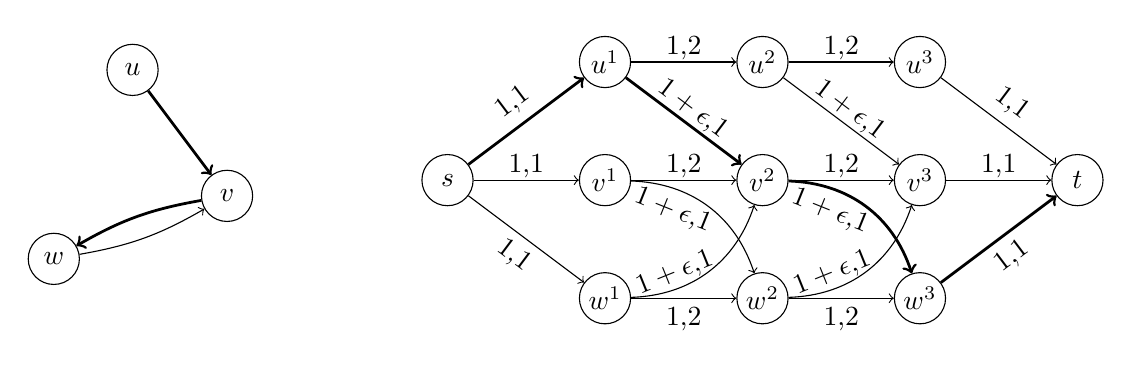
\begin{tikzpicture}[]
\node (w) at (-5,-1) [node] {$w$};
\node (v) at (-2.8,-.2) [node] {$v$};
\node (u) at (-4,1.4) [node] {$u$};

\draw[->, line width=1pt] (u) -- (v);
\draw[->, line width=1pt] (v) to [bend right=10] (w);
\draw[->] (w) to [bend right=10] (v);

\node (s) at (0,0) [node] {$s$};

\node (u1) at (2,1.5) [node] {$u^1$};
\node (v1) at (2,0) [node] {$v^1$};
\node (w1) at (2,-1.5) [node] {$w^1$};

\node (u2) at (4,1.5) [node] {$u^2$};
\node (v2) at (4,0) [node] {$v^2$};
\node (w2) at (4,-1.5) [node] {$w^2$};

\node (u3) at (6,1.5) [node] {$u^3$};
\node (v3) at (6,0) [node] {$v^3$};
\node (w3) at (6,-1.5) [node] {$w^3$};

\node (t) at (8,0) [node] {$t$};


\draw[->, line width=1pt] (s) -- (u1) node [midway, above, sloped] { 1,1 };
\draw[->] (s) -- (v1) node [midway, above=-1mm] { 1,1 };
\draw[->] (s) -- (w1) node [midway, below, sloped] { 1,1 };
\draw[->] (u3) -- (t) node [midway, above, sloped] { 1,1 };
\draw[->] (v3) -- (t) node [midway, above=-1mm] { 1,1 };
\draw[->, line width=1pt] (w3) -- (t) node [midway, below, sloped] { 1,1 };

\draw[->] (u1) -- (u2) node [midway, above=-1mm] { 1,2 };
\draw[->] (v1) -- (v2) node [midway, above=-1mm] { 1,2 };
\draw[->] (w1) -- (w2) node [midway, below] { 1,2 };
\draw[->] (u2) -- (u3) node [midway, above=-1mm] { 1,2 };
\draw[->] (v2) -- (v3) node [midway, above=-1mm] { 1,2 };
\draw[->] (w2) -- (w3) node [midway, below] { 1,2 };

\draw[->, line width=1pt] (u1) -- (v2) node [midway, above=-1mm, sloped] { $1+\epsilon$,1 };
\draw[->] (u2) -- (v3) node [midway, above=-1mm, sloped] { $1+\epsilon$,1 };

\draw[->] (v1) to [bend left=35] node [pos=0.3, below, sloped] { $1+\epsilon$,1 } (w2);
\draw[->] (w1) to [bend right=35] node [pos=0.3, above=-.8mm, sloped] { $1+\epsilon$,1 } (v2);
\draw[->, line width=1pt] (v2) to [bend left=35] node [pos=0.3, below, sloped] { $1+\epsilon$,1 } (w3);
\draw[->] (w2) to [bend right=35] node [pos=0.3, above=-.8mm, sloped] { $1+\epsilon$,1 } (v3);

\end{tikzpicture}
\caption{Illustration of our transformation from \textsc{HamiltonPath} to \textsc{ShortestSmoothPath}.
The first arc weight is the smooth weight, the second the volatile weight.
The thick arcs indicate a Hamiltonian path and the corresponding shortest $\epsilon$-smooth path.}
\label{fig:transformation}
\end{figure}

Delling et al. show some relations between SSPP and Knapsack but the complexity remains open in their paper.
In this section, we prove that SSPP is strongly $\mathcal{NP}$-complete for any $\epsilon \in \mathbb{Q}^{>0}$.
We therefore define the decision variant of the problem as follows:
An instance $(G, w, w^*, s, t, k)$ is a \emph{yes} instance of $\epsilon$-\textsc{ShortestSmoothPath-Dec} if and only if there exists a path $P = (s,\dots, t)$ in $G$ with $w^*(P) \leq k$ and $\ubs_w(P) < 1 + \epsilon$.

\begin{theorem}
\textsc{ShortestSmoothPath-Dec} is strongly $\mathcal{NP}$-complete.
\end{theorem}

\begin{proof}
A solution can be verified in polynomial time.
Determining the path weight in $w^*$ takes running time linear in $\mathcal{O}(|P|)$.
To check the UBS, shortest distances have to be computed for all $\mathcal{O}(|P|^2)$ subpaths.
This shows that \textsc{ShortestSmoothPath-Dec} $\in \mathcal{NP}$.

To prove the hardness, we give a reduction from the strongly $\mathcal{NP}$-complete \textsc{HamiltonPath} problem. % TODO cite completeness
The goal is to find a \emph{Hamiltonian} path, i.e. a simple path which traverses every vertex exactly once.
Let $G=(V,A)$ be the \textsc{HamiltonPath} instance.
To distinguish them from the vertices in the SSPP instance, we will denote the vertices in $V$ as \emph{nodes}.
We construct our SSPP instance by replicating the nodes of $G$ into $n$ layers and two additional vertices $s$ and $t$.
We connect successive layers with the original arcs and additional arcs between vertices corresponding to the same node.
Any $(s,\dots,t)$ path has exactly $|V|+1$ arcs and has to traverse all layers.
We will choose the arc weights in such a way that the shortest $\epsilon$-smooth path between $s$ and $t$ has to use a different node in each layer.
Paths using the same node in different layers will always be non-$\epsilon$-smooth in $w$ or too long in $w^*$.

Formally, we construct the graph $G'=(V',A')$ for our SSPP instance as follows:
We set the vertices $V' = \{ v^i \mid v \in V, i \in [1,n] \} \cup \{s,t\}$.
The arc set $A'$ is the union of three groups of arcs $A_{\operatorname{orig}}$, $A_{\operatorname{self}}$ and $A_{\operatorname{terminal}}$ where $A_{\operatorname{orig}} = \{ (u^i, v^{i+1}) \mid uv \in A, 1 \leq i < n \}$ are the arcs between the layers corresponding to arcs in the \textsc{HamiltonPath} instance, $A_{\operatorname{self}} = \{ (v^i, v^{i+1}) \mid v \in V, 1 \leq i < n \}$ are the additional arcs between the same nodes in successive layers and $A_{\operatorname{terminal}} = \{ (s, v^1) \mid v \in V \} \cup \{ (v^n, t) \mid v \in V \}$ are the arcs connecting the terminals with the first and last layer.
In both weight functions, all arcs in $A_{\operatorname{terminal}}$ get the weight 1.
The arcs in $A_{\operatorname{self}}$ get a volatile weight of 2 and a smooth weight of 1.
The arcs in $A_{\operatorname{orig}}$ get a volatile weight of 1 and a smooth weight of $1+\epsilon$.
Setting $k=|V|+1$, this forms our \textsc{ShortestSmoothPath-Dec} instance.
This transformation has quadratic running time.
See Figure~\ref{fig:transformation} for an illustrated example of the construction.
For the sake of readability, we use non-integer weights of $1+\epsilon$ in this proof.
The weights can be turned into integers by multiplying them with the denominator of $\epsilon$.

Now, assume that the \textsc{HamiltonPath} instance admits a Hamiltonian path $P = (v_1, \dots, v_n)$.
Then, $P' = (s, v_1^1, \dots, v_n^n, t)$ is a solution to the SSPP problem.
The path uses two arcs from $A_{\operatorname{terminal}}$ and $|V|-1$ arcs from $A_{\operatorname{orig}}$.
Thus, $w^{*}(P') = |V| + 1 = k$.
Also, its $\ubs_w(P')$ must be smaller than $1+\epsilon$.
Due to Observation~\ref{obs:append_sp_ubs}, it is sufficient to show that the UBS is small enough for $P'' = (v_1^1, \dots, v_n^n)$.
For any subpath $P''_{i,j} = (u^i, \dots v^j)$ for $i < j$, $u$ must not be equal to $v$ because $P$ is a Hamiltonian path.
As all arcs are from $A_{\operatorname{orig}}$, $w(P''_{i,j}) = (j-i) \cdot (1+\epsilon)$.
The shortest path (with respect to $w$) between $u^i$ and $v^j$ has to use at least one $A_{\operatorname{orig}}$ arc because $u \neq v$.
Thus, $\dist_w(P''_{i,j}) \geq (i - j - 1) + (1 + \epsilon)$.
This yields
\[
\ubs_w(P''_{i,j}) = \frac{w(P''_{i,j})}{\dist_w(P''_{i,j})} \leq \frac{(j-i) \cdot (1+\epsilon)}{j-i+\epsilon} < \frac{(j-i) \cdot (1+\epsilon)}{j-i} = 1 + \epsilon
\]
which proves that $P'$ is valid solution for the SSPP instance.

Conversely, suppose that our SSPP instance has an $\epsilon$-smooth path $P' = (s, v_1^1, \dots, v_n^n, t)$ of weight $w^*(P') = |V|+1$.
Such a path cannot contain any arcs from $A_{\operatorname{self}}$ because their volatile weight is 2.
We now show that no two vertices in the path can correspond to the same node and thus that $P = (v_1, \dots, v_n)$ is indeed a Hamiltonian path in $G$.
Suppose for contradiction that $P'_{i,j} = (v^i, \dots, v^j)$ was a subpath of $P'$.
The length $w(P'_{i,j})$ is $(i-j) \cdot (1+\epsilon)$.
Since start and end vertex correspond to the same node, the shortest path with respect to $w$ between these vertices is made up of arcs from $A_{\operatorname{self}}$ and has distance $\dist_w(v^i, v^j) = i-j$.
Thus, $\ubs_w(P'_{i,j}) = (1+\epsilon)$ which means that this subpath must not be part of a solution for the SSPP instance.
This is a contradiction.
Thus, the SSPP solution induces a valid solution for the \textsc{HamiltonPath} instance.
\end{proof}

\section{Algorithms}\label{sec:algos}

Delling et al. propose the Iterative Path Blocking (IPB) algorithm to solve the SSPP optimally.
The algorithm repeats two steps until a valid path is found.
It maintains a set of blocked paths, which is initially empty.
In the first step, a shortest path with regards to $w^*$ is computed while avoiding any blocked paths.
In the second step, the obtained path is checked for subpaths violating the UBS constraint.
Any violating subpaths are added to the list of blocked paths and the algorithm continues with the next iteration.
If no violating subpath is found, the final path is returned.

This framework can be implemented with different concrete algorithms for both steps.
The implementation described in~\cite{dss-tarrn-18} is based on CRP~\cite{dgpw-crprn-13}.
In this paper, we propose optimized implementations for both steps based on Lazy RPHAST and (C)CH-Potentials.

\subsection{Avoiding Blocked Paths}\label{sec:ipb}

\begin{figure}
\centering
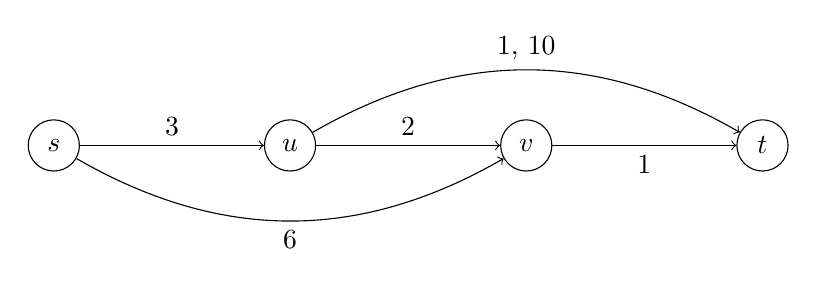
\begin{tikzpicture}[]
\node (s) at (0,0) [node] {$s$};
\node (u) at (3,0) [node] {$u$};
\node (v) at (6,0) [node] {$v$};
\node (t) at (9,0) [node] {$t$};

\draw[->] (s) -- (u) node [midway, above] { 3 };
\draw[->] (u) -- (v) node [midway, above] { 2 };
\draw[->] (v) -- (t) node [midway, below] { 1 };

\draw[->] (s) to [bend right=30] node [midway, below] { 6 } (v);
\draw[->] (u) to [bend left=30] node [midway, above] { 1, 10 } (t);
\end{tikzpicture}
\caption{Example graph where for $\epsilon = 1$ the shortest $\epsilon$-smooth path $(s,v,t)$ is not prefix-optimal. For all arcs except $ut$, the smooth and the volatile metric are equal. For $uv$, the smooth weight is 1 and the volatile weight 10.}
\label{fig:ipb_counterexample}
\end{figure}

Delling et al. describe their approach to the first phase as a variant of Dijkstra's algorithm.
When relaxing an arc $uv$ where $v$ is the endpoint of a blocked path, they backtrack the parent pointers of $v$, comparing the reconstructed path to the blocked path.
Should the paths match, the search is pruned at $v$.
This algorithm correctly avoids blocked paths.
However, it also avoids some additional paths because Dijkstra's algorithm by construction only finds prefix-optimal paths.
But optimal shortest smooth paths may not be prefix-optimal with respect to the volatile metric $w^*$.
See Figure~\ref{fig:ipb_counterexample} for an example.
To the best of our understanding, IPB as described by Delling et al. will not find the shortest smooth path in this example.
The algorithm will find the path $(s,u,v,t)$ in the first iteration.
This path is not 1-smooth because $(u,v,t)$ has stretch 3 and $(u,v,t)$ will be added to the blocked path set.
With $(u,v,t)$ blocked, the algorithm will find the path $(s,u,t)$ in the next iteration and return it as the final result.
However, the shortest 1-smooth path is $(s,v,t)$.
It was missed because the prefix $(s,v)$ is not optimal in $w^*$ and was therefore pruned at $v$ by $(s,u,v)$.
We will refer to this variant from now on by \emph{heuristic iterative path blocking} (IPB-H).
IPB-H will still find an $\epsilon$-smooth path though it may not necessarily be the shortest.
Therefore, it is only a heuristic for the SSPP.

To guarantee to find shortest smooth path with Dijkstra's algorithm, we need to adjust the notion of optimality used to compare labels.
It might be necessary to keep a label with sub-optimal distance from the start as in the example from Figure~\ref{fig:ipb_counterexample} where the label for $(s,v)$ needs to be kept at $u$ despite being longer than $(s,u,v)$.
This leads to a \emph{label-correcting} variation of Dijkstra's algorithm with the possibility for multiple labels per vertex.
A \emph{label} $l$ at a vertex $v$ consists of a distance from the source $\mathtt{D}_l$, a set of active blocked paths $\mathtt{A}_l$, and a pointer to the parent vertex and label for efficient reconstruction of the path $P(l) = (s,\dots,v)$ represented by the label.
The active blocked path set $\mathtt{A}_l$ contains all blocked paths which have a prefix which is a suffix of $P(l)$.
A label $l$ can be discarded when $v$ has another label $l'$ with $\mathtt{D}_{l'} \leq \mathtt{D}_l$ and $\mathtt{A}_{l'} \subseteq \mathtt{A}_l$.

The search is initialized with a single label at $s$ with distance zero and an empty set of active blocked paths.
When a vertex $u$ with a label $l_u$ is popped from the queue and an arc $uv$ is relaxed, we create a new label $l_v$ as follows:
We set the distance $\mathtt{D}_{l_v} = \mathtt{D}_{l_u} + w^*(uv)$ and the parent label to $l_u$.
We also need to keep track of traversed blocked paths.
If $uv$ is the first arc of a blocked path $B = (u,v,\dots)$, the path $B$ needs to be added to $\mathtt{A}_{l_v}$.
For any active blocked path $B = (\dots, u, w, \dots) \in \mathtt{A}_{l_u}$, we need to check if $w=v$, i.e. $uv$ lies on $B$.
If this is the case, $B$ is contained in $\mathtt{A}_{l_v}$, or, if $uv$ is the last arc of $B$, the label $l_v$ must be dropped.
If $uv$ is not on $B$, the blocked path is not in $\mathtt{A}_{l_v}$.

An efficient implementation of this algorithm requires careful engineering.
For each arc, we keep track of the blocked paths it lies on.
Labels use a bitset to store the active blocked paths.
The bitsets are limited to the paths relevant for the current vertex.
This allows for efficient subset checks with bit-wise operations.
Additionally, each vertex maintains its own queue of labels ordered by distance from $s$.
When the vertex is popped from the queue, it pops the next label from its queue and propagates only this label.
If there are any remaining labels in the queue, the vertex is reinserted into the global queue.
Finally, we utilize A* with CCH-Potentials on the volatile metric to guide the search towards the target.
As our experiments show, disallowing non $\epsilon$-smooth paths increase distances only very little.
Thus, the heuristic is close to perfect and A* very effective for this problem.

\subsection{Efficient UBS Computation}\label{sec:ubs_tree}

\begin{figure}
\centering
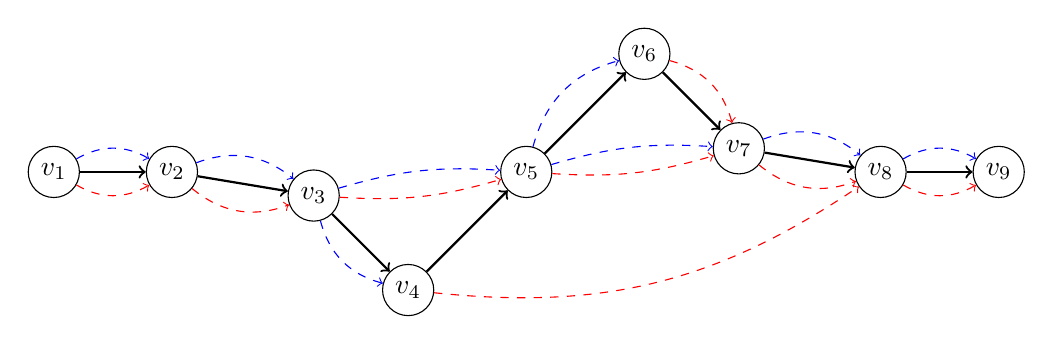
\begin{tikzpicture}[]
\node (s) at (0,0) [node]      {$v_1$};
\node (1) at (1.5,0) [node]    {$v_2$};
\node (2) at (3.3,-0.3) [node] {$v_3$};
\node (3) at (4.5,-1.5) [node] {$v_4$};
\node (4) at (6,0) [node]      {$v_5$};
\node (5) at (7.5,1.5) [node]  {$v_6$};
\node (6) at (8.7,0.3) [node]  {$v_7$};
\node (7) at (10.5,0) [node]   {$v_8$};
\node (t) at (12,0) [node]     {$v_9$};

\draw[->, thick] (s) -- (1);
\draw[->, thick] (1) -- (2);
\draw[->, thick] (2) -- (3);
\draw[->, thick] (3) -- (4);
\draw[->, thick] (4) -- (5);
\draw[->, thick] (5) -- (6);
\draw[->, thick] (6) -- (7);
\draw[->, thick] (7) -- (t);

\draw[->, dashed, blue] (s) to [bend left=30] (1);
\draw[->, dashed, blue] (1) to [bend left=30] (2);
\draw[->, dashed, blue] (2) to [bend right=30] (3);
\draw[->, dashed, blue] (2) to [bend left=10] (4);
\draw[->, dashed, blue] (4) to [bend left=30] (5);
\draw[->, dashed, blue] (4) to [bend left=10] (6);
\draw[->, dashed, blue] (6) to [bend left=30] (7);
\draw[->, dashed, blue] (7) to [bend left=30] (t);


\draw[->, dashed, red] (7) to [bend right=30] (t);
\draw[->, dashed, red] (6) to [bend right=30] (7);
\draw[->, dashed, red] (3) to [bend right=20] (7);
\draw[->, dashed, red] (5) to [bend left=30] (6);
\draw[->, dashed, red] (4) to [bend right=10] (6);
\draw[->, dashed, red] (2) to [bend right=10] (4);
\draw[->, dashed, red] (1) to [bend right=30] (2);
\draw[->, dashed, red] (s) to [bend right=30] (1);
\end{tikzpicture}
\caption{Example path (solid, black) with shortest path tree from $v_1$ to all vertices on the path (dashed, blue) and reverse shortest path tree from all vertices on the path to $v_9$ (dashed, red).}
\label{fig:ubs_tree}
\end{figure}

According to Delling et al.~\cite{dss-tarrn-18}, the UBS computation is one of the bottlenecks of the IPB approach.
They employ a many-to-many algorithm.
Computing the UBS has been studied before in the context of alternative route algorithms~\cite{adgw-arrn-13}.
There, the authors state that it would be ideal to check the UBS in time proportional to the length of the path and a few shortest path queries.
% Due to the lack of such an option they resort to approximations.
Here, we introduce an algorithm which achieves this when possible.
We also prove that this is not always possible by constructing a worst-case example where each subpath has a distinct stretch value.

Consider a path $P=(s=v_1,\dots,t=v_k)$ as depicted in Figure~\ref{fig:ubs_tree}.
Our algorithm works iteratively.
We start with the full path and successively remove prefixes and suffixes until the path is empty or only a shortest path remains.
We start by computing shortest distances from $s$ to all vertices on the path.
This can be done with a single run of Dijkstra's algorithm which can terminate once all $v_i$ have been settled.
Beside the shortest distances, this yields a shortest path tree represented though parent pointers.
We also run Dijkstra's algorithm from $t$ on the reversed graph which yields a backward shortest path tree to $t$.
Now we find the greatest index $i$ such that $P_{1,i}$ is a prefix of all shortest paths $\shp(s, v_l)$ where $i < l \leq k$, i.e. the first branching vertex in the forward shortest path tree.
In the worst case this may be $s$.
In the example in Figure~\ref{fig:ubs_tree} this is $v_3$.
We analogously obtain the first branching vertex in the reverse shortest path tree to $v_k$ ($v_8$ in our example).
Stated formally, this is the smallest index $j$ such that $P_{j,k}$ is a suffix of all shortest paths $\shp(v_l, t)$ where $1 \leq l \leq j$.
% how to find? early termination
By Observation~\ref{obs:append_sp_ubs} subpaths starting from vertices in the segment $P_{1,i-1}$ and subpaths ending at vertices from $P_{j+1,k}$ are not relevant to the UBS computation.
% Checking the stretch for subpaths $P_{j,l}$ where $j < i, i < l \leq k$ is not necessary.
We exploit this and only check paths starting from $v_i$ or ending at $v_j$ in the current iteration.

We check the stretch of all subpaths $P_{i,l}$ where $i < l \leq j$ with a linear sweep over the $v_l$.
Since $P_{1,i}$ is a prefix of all shortest paths from $s$, we can compute the distance $\dist(v_i, v_l)$ as $\dist(s, v_l) - \dist(s, v_i)$.
Thus, each stretch can be checked in constant time with the distances computed by Dijkstra's algorithm.
When we are only interested in violating subpaths (rather than computing the exact UBS value of $P$), the sweep can be stopped after the first (i.e. shortest) violating segment has been found.
Forbidding the shortest violating segment starting at $v_i$ is sufficient because it is contained in all longer segments.
Checking the stretches of the subpaths $P_{l,j}$ where $i \leq l < j$ works analogously.

Having checked all these stretches, we continue with the next iteration by applying the whole algorithm to the subpath $P_{i+1,j-1}$.
We can stop when $i+1 \geq j-1$ or when the whole considered path is a shortest path between its endpoints.

% filtering covered

This algorithm can be adopted to efficiently compute other path quality measures such as the \emph{local optimality}~\cite{adgw-arrn-13}.

\subsubsection{Worst-Case Running Time}

This algorithm performs great when large segments are shortest paths, which will of course often be the case when searching shortest smooth paths.
In the worst case however, it still has to check $\Theta(n^2)$ subpath stretches.
Consider a complete graph with unit weights and the path $P=(v_1, \dots, v_n)$.
In this graph the shortest path between any two vertices is always the direct arc and the distance is always exactly one.
Thus, the shortest path tree from any vertex is just a star with the direct arcs and our algorithm can only advance by a single vertex in each iteration.
This results in a worst case running time of $n$ runs of Dijkstra's algorithm.

We suspect that it is not possible to compute the UBS asymptotically faster.
Consider the same graph as before but with weights of unique powers of two for the arcs of the path.
Now any subpath has a unique length.
As all subpaths of three or more vertices still have a shortest distance of one between their endpoints, we have $\Theta(n^2)$ unique stretch values.
Thus, computing the UBS of the whole path without checking all $\Theta(n^2)$ stretch values should be difficult if not impossible.

\subsubsection{Lazy RPHAST with Path Unpacking}
\label{sec:lazy_rphast_path}

\begin{algorithm2e}[t]
\KwData{$\mathtt{P}[u]$: parent vertex on the shortest path from $u$ to $t$, as computed by Algorithm~\ref{algo:lazy_rphast}}
\KwData{$\mathtt{U}[u]$: whether the path from $u$ to $t$ has been fully unpacked}
\SetKwFunction{Dist}{ComputeAndMemoizeDist}
\SetKwFunction{Unpack}{Unpack}
\SetKw{True}{true}
\SetKwProg{Fn}{Function}{:}{}

\Fn{$\Unpack(u)$}{
    \If{$\neg (\mathtt{U}[u] \lor u = t)$}{
        $\Dist(u)$\;
        $\Unpack(\mathtt{P}[u])$\;

        \If{$(u, \mathtt{P}[u])$ is a shortcut for $(u, v, \mathtt{P}[u])$}{
            $\mathtt{P}[v] \leftarrow \mathtt{P}[u]$\;
            $\Unpack(v)$\;
            $\mathtt{P}[u] \leftarrow w$\;
            $\Unpack(u)$\;
        }
        $\mathtt{U}[u] \leftarrow \True$\;
    }
}
\caption{Path unpacking for Lazy RPHAST}
\label{algo:lazy_rphast_path}
\end{algorithm2e}

While this algorithm typically needs few stretch checks, running Dijkstra's algorithm a couple of times is still prohibitively slow on large road networks.
Luckily, we can speed these computations up drastically by employing Lazy RPHAST, which we already used as a A* heuristic in the shortest path search phase.
Recall that Lazy RPHAST allows us to select one target vertex and then to compute shortest distances quickly from many vertices to this target.
For the efficient UBS computation, we use two instantiations of this algorithm.
In each iteration, we select both endpoints of the considered path and compute distances from and to the endpoints for all vertices on the path.
However, we also need the shortest path trees.
We propose an extension to Lazy RPHAST to incrementally compute shortest path trees.

We extend the original Lazy RPHAST algorithm~\ref{algo:lazy_rphast} by additionally storing parent pointers for path unpacking similar to Dijkstra's algorithm.
Thus, after having called \texttt{ComputeAndMemoizeDist}, we have the shortest path through the CH search space.
Algorithm~\ref{algo:lazy_rphast_path} depicts the routine to efficiently unpack shortcuts on this path and retrieve full shortest path trees in the original graph.
We use a bitvector $\mathtt{U}$ to mark vertices for which the shortest path has already been fully unpacked which is checked before any actual work is performed.
Then, we have to call \texttt{ComputeAndMemoizeDist} to ensure that the path through the CH search space has been obtained for $u$.
For vertices encountered through recursive shortcut unpacking this might have not happened before.
In the next step, we can now recursively unpack the full path up to the parent $\mathtt{P}[u]$ of our current vertex $u$.
Now, all that remains is to unpack the arc $(u, \mathtt{P}[u])$ if it is a shortcut.
If so, the middle vertex $v$ is set in $\mathtt{P}$ as the vertex between $u$ and $\mathtt{P}[u]$ and \texttt{Unpack} is invoked recursively first for $v$ and then again for $u$ to unpack the arcs $(v, \mathtt{P}[v])$ and $(u,v)$.

\subsection{Iterative Path Fixing}

With an efficient algorithm to find UBS-violating segments we can introduce another natural heuristic to find short smooth paths:
Find the shortest path with respect to $w^*$ and replace all UBS violating subpaths $(v_i,\dots,v_j)$ with $\shp_w(v_i, v_j)$.
The result may still contain UBS violating subpaths.
In this case, we iteratively continue to replace violating segments.
When a path contains overlapping violating subpaths, we replace the first, ignore following overlapping subpaths and continue with the next non-overlapping segment.
We denote this algorithm as \emph{iterative path fixing} (IPF).

\section{Evaluation}\label{sec:eval}

In this section, we present our experimental results.
Our benchmark machine runs openSUSE Leap 15.3 (kernel 5.3.18), and has 192\,GiB of DDR4-2666 RAM and two Intel Xeon Gold 6144 CPUs, each of which has eight cores clocked at 3.5\,GHz and 8~$\times$~64\,KiB of L1, 8~$\times$~1\,MiB of L2, and 24.75\,MiB of shared L3 cache.
All running times are sequential.
We implement our algorithms in Rust\footnote{The code for this paper and all experiments is available at \url{https://github.com/kit-algo/traffic-aware}} and compile them with \texttt{rustc 1.58.0-nightly (b426445c6 2021-11-24)} in the release profile with the \texttt{target-cpu=native} option.

\begin{table}
\centering
\caption{
Instances used in the evaluation with sequential preprocessing running times to construct a CCH-Potential.
Phase 1 needs to be run only once for each graph, Phase 2 once for each metric, or when a metric changes.
}\label{tab:graphs}
\begin{tabular}{lrrrr}
\toprule
 & Vertices       & Edges          & \multicolumn{2}{c}{Preprocessing [s]} \\ \cmidrule(lr){4-5} & $[\cdot 10^6]$ & $[\cdot 10^6]$ & Phase 1 & Phase 2 \\
\midrule
DIMACS Europe &       18.0 &       42.2 &        2\,260.7 &          11.3 \\
OSM Europe    &      173.8 &      348.0 &        4\,270.0 &          58.8 \\
OSM Germany   &       11.1 &       26.2 &        1\,314.0 &           7.5 \\
\bottomrule
\end{tabular}


\end{table}

Table~\ref{tab:graphs} shows the road networks we use in our experiments alongside sequential preprocessing times.
OSM Europe is the same network used in~\cite{dss-tarrn-18} and publicly available\footnote{\url{https://i11www.iti.kit.edu/resources/roadgraphs.php}}.
The DIMACs Europe instance was made available by PTV\footnote{\url{https://ptvgroup.com}} for the 9th DIMACS implementation challenge~\cite{DemetrescuGJ09}.
It is not publicly available but can be obtained on request for research purposes\footnote{\url{https://i11www.iti.kit.edu/resources/roadgraphs.php}}.
We derived the OSM Germany instance from an early 2020 snapshot of OpenStreetMap and converted into a routing graph using RoutingKit\footnote{\url{https://github.com/RoutingKit/RoutingKit}}.
For this instance, we have proprietary traffic data provided by Mapbox\footnote{\url{https://mapbox.com}} which, unfortunately, we cannot provide.
The data includes two live traffic snapshots in the form of OSM node id pairs and live speeds for the edge between the vertices.
One is from Friday 2019/08/02 afternoon and contains 320K vertex pairs and the other from Tuesday 2019/07/16 morning and contains 185K pairs.
For the Europe instances, we do not have any real world traffic data.
Thus, we resort to the approach suggested in~\cite{dss-tarrn-18} and generate synthetic live traffic:
For each road where the average speed is greater than 30\,kph, we reduce the speed to 5\,kph with a probability of 0.5\%.

We evaluate our algorithms by performing batches of point-to-point shortest $\epsilon$-smooth path queries.
As the distance between source and target has a significant influence on the performance, we generate different query batches.
For each batch, we pick 1000 source vertices uniformly at random.
We then run Dijkstra's algorithm from each source vertex on the graph with the smooth metric.
Following the Dijkstra rank methodology, we store every $2^i$th settled vertex~\cite{ss-hhhes-05}.
This allows evaluating the performance development against varying path lengths.
In~\cite{adgw-arrn-13}, 1-hour queries were performed.
For comparison, we also generate an \emph{1h} batch by picking the first settled vertex with a distance greater than one hour.
In addition we generate a \emph{4h} batch for medium-range queries with the same method and a \emph{random} batch for long range queries where the target is picked uniformly at random.

Preliminary experiments showed that some queries take prohibitively long to answer exactly.
Since we are solving an $\mathcal{NP}$-hard problem, this is not surprising.
We abort queries if the algorithm has not found a path with $\ubs < (1+\epsilon)$ after 10 seconds.
We report these queries as failed but, nevertheless, do include their running times in our measurements.

\begin{figure}
\centering
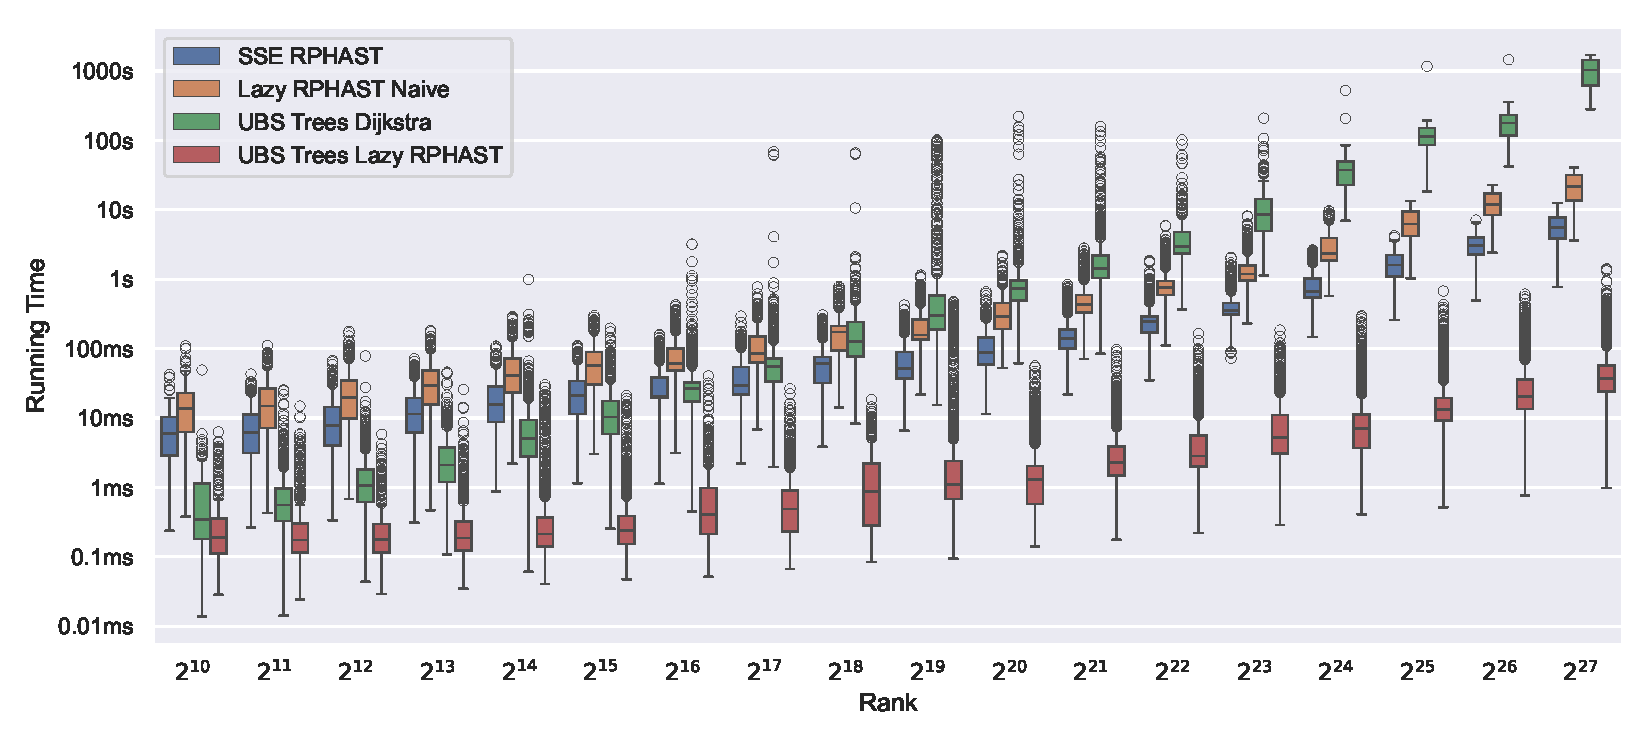
\includegraphics[width=\linewidth]{fig/ubs_perf.pdf}
\caption{
Running times of different UBS checking algorithms for paths encountered by IPB-H when answering queries of different ranks with $\epsilon = 0.2$ on OSM Europe.
The boxes cover the range between the first and third quartile.
The band in the box indicates the median, the whiskers cover 1.5 times the interquartile range.
All other running times are indicated as outliers.
}\label{fig:ubs_perf}
\end{figure}

We start by evaluating different UBS algorithms in isolation.
The paths checked by the UBS algorithms are the paths we find while performing IPB-H to find shortest smooth paths with $\epsilon = 0.2$ on the Dijkstra rank queries.
We limit the time per rank and UBS algorithm to one hour.
Thus, slow algorithms may not get to check all paths.
Our baseline is computing all distances between pairs of path vertices at once with \emph{SSE RPHAST}~\cite{dgw-fbspr-11}, which to the best of our knowledge is the fastest known many-to-many algorithm.
The second algorithm, denoted as~\emph{Lazy RPHAST Naive}, uses Lazy RPHAST to compute distances between all pairs of path vertices.
The third one is \emph{UBS Trees Dijkstra} which is the non-accelerated, i.e. Dijkstra-based, implementation of the efficient UBS computation introduced in Section~\ref{sec:ubs_tree}.
\emph{UBS Trees Lazy RPHAST} denotes the accelerated variant of this algorithm utilizing Lazy RPHAST as described in Section~\ref{sec:lazy_rphast_path}.

Figure~\ref{fig:ubs_perf} depicts the results of our experiment.
We observe that SSE RPHAST is consistently faster than the naive Lazy RPHAST variant by a roughly constant factor.
SSE RPHAST was designed as a many-to-many algorithm and is thus more efficient than naively applying a many-to-one algorithm $|P|$ times.
The non-accelerated UBS Trees algorithm is very fast for short paths but quickly becomes prohibitively slow for longer paths.
Running Dijkstra's algorithm will traverse a large part of the network if source and target are sufficiently far apart from each other.
Doing this multiple times is not feasible.
However, the accelerated variant beats SSE RPHAST by about two orders of magnitude across all path lengths.
UBS Trees running times have significantly greater variance than the many-to-many algorithms.
This is because the amount of work which UBS Trees can avoid varies strongly between different paths.
In contrast, the many-to-many-based algorithms will always check $\mathcal{O}(|P|^2)$ subpath distances.
Note that the UBS Trees Dijkstra outliers disappear because we limit the time per rank and algorithm.
If we checked all paths, the outliers would be present too, but the experiment would take prohibitively long.

\begin{table}
\centering
\caption{
Average performance of our implementations of IPB-E, IPB-H and IPF for different query sets on all instances with $\epsilon = 0.2$.
The Increase column denotes the length increase with respect to $w^*$ of the obtained path over $\shp_{w^*}$ and includes only successful queries.
The running time column also includes the running time of queries aborted after 10 seconds.
}\label{tab:data}
\setlength{\tabcolsep}{4pt}
\begin{tabular}{llrrrrrrrrrr}
\toprule
 & & \multicolumn{2}{c}{Increase $[\%]$} & \multicolumn{2}{c}{Iterations} & \multicolumn{2}{c}{Blocked Paths} & \multicolumn{2}{c}{Time [ms]} & \multicolumn{2}{c}{Failed $[\%]$} \\
\cmidrule(l{3pt}r{3pt}){3-4} \cmidrule(l{3pt}r{3pt}){5-6} \cmidrule(l{3pt}r{3pt}){7-8} \cmidrule(l{3pt}r{3pt}){9-10} \cmidrule(l{3pt}r{3pt}){11-12}
 & & IDB & IPB & IDB & IPB & IDB & IPB & IDB & IPB & IDB & IPB \\
\midrule
\multirow{4}{*}{\rotatebox[origin=c]{90}{1h}} & DIMACS Eur Syn &                     3.6 &  1.0 &            6.9 &   33.0 &                24.5 &   98.8 &           108.4 &    29.4 &    1.6 &  10.5 \\
                & OSM Eur Syn &                     0.3 &  0.2 &            1.8 &   11.0 &                 1.4 &   39.7 &             3.7 &     9.0 &    0.2 &   2.2 \\
                & OSM Ger Fri &                     1.7 &  0.3 &            8.3 &   48.8 &                44.2 &  123.3 &           191.5 &    71.6 &    1.1 &  17.7 \\
                & OSM Ger Tue &                     0.3 &  0.1 &            1.7 &   13.6 &                 4.4 &   33.8 &            10.8 &    16.7 &    0.0 &   3.9 \\
\addlinespace \multirow{4}{*}{\rotatebox[origin=c]{90}{4h}} & DIMACS Eur Syn &                     3.8 &  1.2 &           16.2 &  115.3 &                75.0 &  479.5 &           354.6 &   301.3 &    3.1 &  41.1 \\
                & OSM Eur Syn &                     0.3 &  0.2 &            3.1 &   36.6 &                 4.8 &  155.2 &            28.2 &    68.5 &    0.6 &   7.3 \\
                & OSM Ger Fri &                     3.3 &  0.3 &           51.5 &  179.2 &               407.4 &  531.8 &          6\,631.5 &  1\,000.9 &    8.4 &  69.8 \\
                & OSM Ger Tue &                     0.4 &  0.1 &            4.3 &   49.7 &                23.0 &  147.0 &           105.3 &   141.5 &    0.0 &  17.4 \\
\addlinespace \multirow{4}{*}{\rotatebox[origin=c]{90}{Random}} & DIMACS Eur Syn &                     3.5 &  1.1 &           45.6 &  189.3 &               222.2 &  909.7 &         10\,515.9 &  7\,656.5 &   11.8 &  71.6 \\
                & OSM Eur Syn &                     0.3 &  0.2 &           11.5 &  140.3 &                30.1 &  875.5 &           662.3 &  9\,713.8 &    3.1 &  43.2 \\
                & OSM Ger Fri &                     3.1 &  0.3 &           47.9 &  158.3 &               386.7 &  469.0 &          9\,567.2 &   926.0 &    8.8 &  61.7 \\
                & OSM Ger Tue &                     0.4 &  0.1 &            4.1 &   45.4 &                24.5 &  126.7 &           132.5 &   139.4 &    0.0 &  16.3 \\
\bottomrule
\end{tabular}

\end{table}

Next, we evaluate the performance of our query algorithms on realistic queries and instances.
Table~\ref{tab:data} depicts the results.
Both the query set and the instance have a strong influence on the running time.
Note that random queries on OSM Germany are on average shorter than four hours which is the reason why the running times on OSM Germany for random queries are faster than for 4h queries.
The length increase of the solutions primarily depends on the instance and less on the query set.
The synthetic traffic affects DIMACS Europe more strongly than OSM Europe.
We suspect that this is because OSM is modeled in much greater detail and contains more shorter arcs. % which when jammed have less influence when jammed as a single long arc.
In terms of running time, IPB-H is significantly faster than IPB-E and IPF is significantly faster still, which is roughly what we expected.
Conversely, the heuristics find somewhat longer paths than the exact IPB-E algorithm and IPF appears to find worse paths than IPB-H.
However, one has to be careful interpreting these numbers as a non-negligible amount of queries did not terminate with IPB-E and IPB-H.
Because the length increase numbers are averages over different sets, it is not immediately clear if the differences appear because the heuristics find worse paths or because the heuristics find long solutions where the exact algorithm did not finish within 10 seconds.
% When limiting the evaluation to queries where all algorithms finished successfully, the difference between IPB-H and IPB-E almost disappears.
% The gap to IPF also becomes smaller but remains significant.
For running times, the averages are also difficult to interpret.
They are heavily skewed by outliers and there is little reason to assume that they would be normally distributed.
For example, \emph{median} running times for 1h queries of all algorithms on all instances are all below 2\,ms. % and the differences for the other query sets become only more extreme.
Clearly, drawing statistically sound conclusions from this experiment requires a closer look.

\begin{figure}
\centering
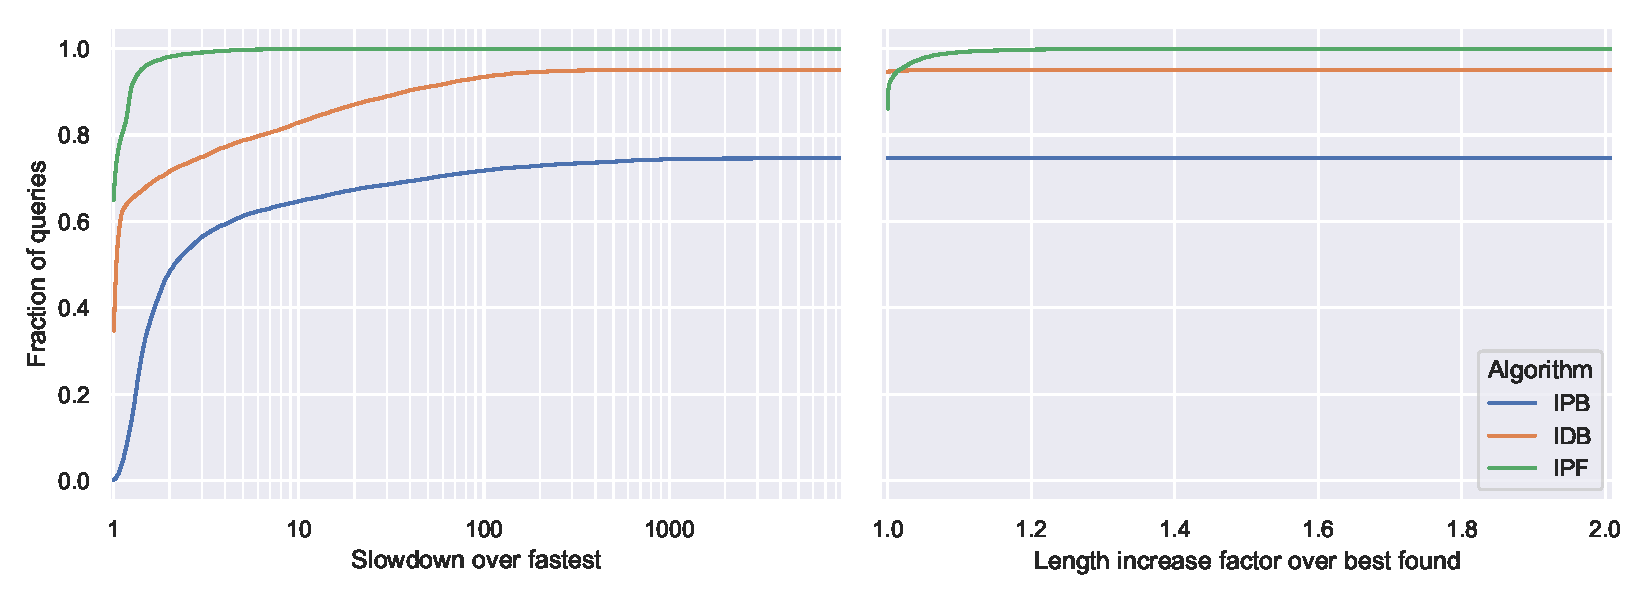
\includegraphics[width=\linewidth]{fig/combined_perf_profile.pdf}
\caption{
Relative performance profiles of our algorithms on all queries from Table~\ref{tab:data}.
}\label{fig:perf_profile}
\end{figure}

Figure~\ref{fig:perf_profile} depicts performance profiles~\cite{dolan2002benchmarking} for running time and found path length of all queries from Table~\ref{tab:data} combined.
Investigating queries across all instances combined is reasonable because we study the relative performance of the different algorithms on each query.
Let $\mathcal{A}$ be the set of algorithms, $\mathcal{Q}$ the set of queries and $\operatorname{obj}(a, q)$ denote the considered measurement from the computation of $a \in \mathcal{A}$ to answer $q \in \mathcal{Q}$.
In our case, this is either the running time or the length with respect to $w^*$ of the computed path.
The performance ratio $r(a,q) = \frac{\operatorname{obj}(a, q)}{\min{\{\operatorname{obj}(a', q) \mid a' \in \mathcal{A}\}}}$ indicates by what factor $a$ deviates from the best solution or the shortest running time for the query $q$.
The performance profile $\rho_a : [1,\infty) \to [0,1], \tau \mapsto \frac{|\{q \in \mathcal{Q} | r(a, q) \leq \tau \}|}{|\mathcal{Q}|}$ of $a$ is the fraction of queries for which $a$ is within a factor of $\tau$ of the best measurement.
For computations that were aborted after 10 seconds, $\operatorname{obj}(a, q) = \infty$.
For the sake of completeness, we also include the same performance profiles separated per instance and query set in the appendix (see Figure~\ref{fig:perf_profile_time} and \ref{fig:perf_profile_quality}).
However, discussing the results in such detail is beyond the scope of this paper.

The running time performance profile in Figure~\ref{fig:perf_profile} allows for some more nuanced observations:
IPF is the fastest algorithm on about 65\% of the queries and almost never more than 10 times slower than the fastest one.
Surprisingly, IPB-H is also sometimes the fastest to answer a query (in 35\% of the queries) but it may also be up to 300 times slower than the fastest algorithm.
However, for 83\% of all queries it stays within a factor of 10.
IPB-H fastest on 35\% and 83\% within factor 10.
The exact algorithm is never the fastest but still within a factor of 10 for 65\% of the queries.
It still may be several thousand times slower than the fastest algorithm in extreme cases, even with the running time limited to 10 seconds.

The path length performance profile also yields useful insights.
Since IPB-E is an exact algorithm, its performance profile contains only a single datapoint, i.e. for all queries which terminated successfully IPB-E finds the shortest path.
The line for IPB-H is almost constant.
This means, there are only few queries where it does not find the best solution.
Even when it does not find the best solution, it is close to the best one, i.e. the maximum length increase factor over the best solution is 1.36 and all other values are below 1.1.
It is quite possible that IPB-H found the optimal solution even for some of the queries where IPB-E did not terminate.
The qualitative performance of IPF varies more strongly.
It also finds the best solution on 85\% of the queries.
More than 99\% of the obtained solutions are within a factor of 1.2 to the best found.
In the worst case IPF found a path 1.96 times the length of the best one found by another algorithm.

In combination with the averages reported in Table~\ref{tab:data} we can now draw solid conclusions on the performance of the algorithms.
IPF is the algorithm with the most stable running time.
Even though it is not always the fastest, it is never much slower than any other algorithm.
It is the only algorithm able to answer all queries in less than 10 seconds.
In fact, it usually needs only a few milliseconds and only up to several hundreds of milliseconds for extreme cases.
It sometimes pays for this with worse solution quality but is still very close to the best found for the vast majority of queries.
This makes it an algorithm suitable for practical applications.
IPB-H is also a very effective heuristic.
It is drastically faster than the exact algorithm and sometimes even faster than IPF.
Its performance in terms of quality is much more stable than IPF and usually IPB-H will find the best path or something very close to it.
The difference in average length increase between IPB-E and IPB-H was not because IPB-H finds much worse paths but because it is able to answer queries which IPB-E cannot answer.
However, it still fails to answer about 5\% of all queries in less than 10 seconds.
The running time of IPB-E varies even more strongly.
On the one hand, many easy queries can be answered in a few milliseconds, but on the other hand, 25\% of all queries cannot be answered in less than 10 seconds.
The feasibility of solving the problem to exactness with IPB-E strongly depends on the distance of queries and on the smoothness of the $w^*$ metric.

\begin{table}[t]
\centering
\caption{
Average performance of our implementations of IPB-E, IPB-H and IPF for different values of $\epsilon$ with 1h queries on OSM Europe with synthetic live traffic.
The Increase column denotes the length increase with respect to $w^*$ of the shortest smooth path over the shortest $w^*$ path.
It includes only values from successful queries.
All other columns indicate average values over all queries, including the ones terminated after 10 seconds.
}\label{tab:epsilon}
\begin{tabular}{clrrrrrrr}
\toprule
            & & Increase & Iterations & Blocked & \multicolumn{3}{c}{Running time [ms]} & Failed \\ \cmidrule(lr){6-8}
 $\epsilon$ & &   $[\%]$ &            &   paths & A* & UBS & Total                      & $[\%]$ \\
\midrule
\multirow{3}{*}{0.01} & IPB-E &                     0.43 &          137.90 &                676.2 &                      307.6 &               22.7 &            335.9 &     2.4 \\
                      & IPB-H &                     0.56 &           22.38 &                 24.9 &                       52.8 &               21.0 &             74.0 &     0.6 \\
                      & IPF &                     0.61 &            1.73 &                    - &                          - &                  - &              2.3 &     0.0 \\[2pt]
\multirow{3}{*}{0.05} & IPB-E &                     0.34 &           68.10 &                351.7 &                      132.5 &               14.8 &            150.3 &     0.9 \\
                      & IPB-H &                     0.39 &           32.78 &                 39.8 &                       19.6 &               38.7 &             58.6 &     0.5 \\
                      & IPF &                     0.41 &            1.54 &                    - &                          - &                  - &              2.3 &     0.0 \\[2pt]
\multirow{3}{*}{0.10} & IPB-E &                     0.27 &           47.35 &                256.4 &                      103.3 &               12.7 &            118.3 &     0.8 \\
                      & IPB-H &                     0.33 &           27.10 &                 27.1 &                        3.5 &               28.9 &             32.7 &     0.3 \\
                      & IPF &                     0.34 &            1.45 &                    - &                          - &                  - &              2.7 &     0.0 \\[2pt]
\multirow{3}{*}{0.20} & IPB-E &                     0.23 &           24.92 &                141.7 &                       51.1 &                7.5 &             59.7 &     0.4 \\
                      & IPB-H &                     0.26 &           19.33 &                 19.0 &                        2.6 &               19.6 &             22.4 &     0.2 \\
                      & IPF &                     0.28 &            1.36 &                    - &                          - &                  - &              2.1 &     0.0 \\[2pt]
\multirow{3}{*}{0.50} & IPB-E &                     0.16 &           13.64 &                 80.0 &                       41.1 &                3.8 &             45.6 &     0.1 \\
                      & IPB-H &                     0.17 &           19.54 &                 18.9 &                        2.5 &               19.4 &             22.1 &     0.2 \\
                      & IPF &                     0.19 &            1.26 &                    - &                          - &                  - &              2.0 &     0.0 \\[2pt]
\multirow{3}{*}{1.00} & IPB-E &                     0.11 &           10.51 &                 55.5 &                       28.1 &                4.4 &             33.4 &     0.2 \\
                      & IPB-H &                     0.12 &           15.13 &                 14.3 &                        2.4 &                9.6 &             12.2 &     0.1 \\
                      & IPF &                     0.14 &            1.19 &                    - &                          - &                  - &              2.5 &     0.0 \\
\bottomrule
\end{tabular}


\end{table}

For our final experiment, we evaluate the performance of our algorithms with different choices for $\epsilon$ with 1000 queries of 1h range on OSM Europe.
Table~\ref{tab:epsilon} depicts the results.
This experiment was also performed in~\cite{dss-tarrn-18} but with only 100 queries.
Given the observation from the previous experiment, it should be clear that reported averages allow only for very rough comparisons.
However, it is the only data available to compare against related work.
Also note that due to the presence of heavy outliers, performing too few queries can distort the numbers drastically.
For example, when we ran the same experiment with only 100 queries, the average running times of IPB-H were an order of magnitude faster.

We observe similar trends as Delling et al.
The smaller the choice of $\epsilon$, the harder the problem becomes.
Consequently, the length increase, the number of iterations, the number of blocked paths and the running time increase.
However, for our implementation of IPB-H, we measure slightly bigger path increases and slightly more iterations.
Our implementation of IPB-H achieves running times two orders of magnitude faster than the CRP-based IPB-H implementation in~\cite{dss-tarrn-18}.
One reason for this is our new UBS algorithm which only needs a couple of milliseconds across all values of $\epsilon$.
In~\cite{dss-tarrn-18}, the UBS checking phase takes between 1.3 and 1.9 \emph{seconds}.
The CH-Potentials based shortest path finding phase is also very efficient across the entire range of $\epsilon$ values.
Even with many blocked paths, the path lengths increase only little and the CH-Potentials heuristic remains very tight and yields good speed-ups.
Our exact IPB-E algorithm is still an order of magnitude faster than the IPB-H implementation in~\cite{dss-tarrn-18}.

\section{Conclusion}

In this paper, we studied the shortest smooth path problem and proved its $\mathcal{NP}$-completeness.
We introduced a new algorithm for practically efficient UBS computation.
This algorithm can compute the exact UBS of typically occurring paths with very few shortest path computations.
It outperforms state-of-the-art exact UBS algorithms by around two orders of magnitude and makes computing exact UBS values feasible in practice.
Also, it can be used for other path quality measures such as local optimality.

We also adapted the existing IPB-H algorithm and realized it with our new UBS algorithm and A* with CH-Potentials.
This realization of IPB-H outperforms the original implementation by two orders of magnitude.
Also, we present necessary modifications to make the algorithm exact.
Our exact version is still about an order of magnitude than the CRP-based heuristic implementation.
As IPB-H and IPB-E are not always able to find solutions in reasonable time, we introduce another heuristic, IPF.
IPF can consistently find smooth paths even for random queries on massive continental sized instances in a few tenths of milliseconds.

For future work we would like to apply our algorithms not only to live traffic but also to predicted traffic, i.e. find smooth paths in a time-dependent setting.
Further, it would be interesting to study what causes IPB-H to be so much faster than IPB-E while retaining most of the quality.
Maybe this could be traced to specific structures in road networks which then in turn could be exploited to speed up IPB-E.
% work around performance problems (circles, expontial number of forb paths - forbid corridors)

% \section{Typesetting instructions -- Summary}
% \label{sec:typesetting-summary}

% LIPIcs is a series of open access high-quality conference proceedings across all fields in informatics established in cooperation with Schloss Dagstuhl.
% In order to do justice to the high scientific quality of the conferences that publish their proceedings in the LIPIcs series, which is ensured by the thorough review process of the respective events, we believe that LIPIcs proceedings must have an attractive and consistent layout matching the standard of the series.
% Moreover, the quality of the metadata, the typesetting and the layout must also meet the requirements of other external parties such as indexing service, DOI registry, funding agencies, among others. The guidelines contained in this document serve as the baseline for the authors, editors, and the publisher to create documents that meet as many different requirements as possible.

% Please comply with the following instructions when preparing your article for a LIPIcs proceedings volume.
% \paragraph*{Minimum requirements}

% \begin{itemize}
% \item Use pdflatex and an up-to-date \LaTeX{} system.
% \item Use further \LaTeX{} packages and custom made macros carefully and only if required.
% \item Use the provided sectioning macros: \verb+\section+, \verb+\subsection+, \verb+\subsubsection+, \linebreak \verb+\paragraph+, \verb+\paragraph*+, and \verb+\subparagraph*+.
% \item Provide suitable graphics of at least 300dpi (preferably in PDF format).
% \item Use BibTeX and keep the standard style (\verb+plainurl+) for the bibliography.
% \item Please try to keep the warnings log as small as possible. Avoid overfull \verb+\hboxes+ and any kind of warnings/errors with the referenced BibTeX entries.
% \item Use a spellchecker to correct typos.
% \end{itemize}

% \paragraph*{Mandatory metadata macros}
% Please set the values of the metadata macros carefully since the information parsed from these macros will be passed to publication servers, catalogues and search engines.
% Avoid placing macros inside the metadata macros. The following metadata macros/environments are mandatory:
% \begin{itemize}
% \item \verb+\title+ and, in case of long titles, \verb+\titlerunning+.
% \item \verb+\author+, one for each author, even if two or more authors have the same affiliation.
% \item \verb+\authorrunning+ and \verb+\Copyright+ (concatenated author names)\\
% The \verb+\author+ macros and the \verb+\Copyright+ macro should contain full author names (especially with regard to the first name), while \verb+\authorrunning+ should contain abbreviated first names.
% \item \verb+\ccsdesc+ (ACM classification, see \url{https://www.acm.org/publications/class-2012}).
% \item \verb+\keywords+ (a comma-separated list of keywords).
% \item \verb+\relatedversion+ (if there is a related version, typically the ``full version''); please make sure to provide a persistent URL, e.\,g., at arXiv.
% \item \verb+\begin{abstract}...\end{abstract}+ .
% \end{itemize}

% \paragraph*{Please do not \ldots} %Do not override the \texttt{\seriesstyle}-defaults}
% Generally speaking, please do not override the \texttt{lipics-v2021}-style defaults. To be more specific, a short checklist also used by Dagstuhl Publishing during the final typesetting is given below.
% In case of \textbf{non-compliance} with these rules Dagstuhl Publishing will remove the corresponding parts of \LaTeX{} code and \textbf{replace it with the \texttt{lipics-v2021} defaults}. In serious cases, we may reject the LaTeX-source and expect the corresponding author to revise the relevant parts.
% \begin{itemize}
% \item Do not use a different main font. (For example, the \texttt{times} package is forbidden.)
% \item Do not alter the spacing of the \texttt{lipics-v2021.cls} style file.
% \item Do not use \verb+enumitem+ and \verb+paralist+. (The \texttt{enumerate} package is preloaded, so you can use
%  \verb+\begin{enumerate}[(a)]+ or the like.)
% \item Do not use ``self-made'' sectioning commands (e.\,g., \verb+\noindent{\bf My+ \verb+Paragraph}+).
% \item Do not hide large text blocks using comments or \verb+\iffalse+ $\ldots$ \verb+\fi+ constructions.
% \item Do not use conditional structures to include/exclude content. Instead, please provide only the content that should be published -- in one file -- and nothing else.
% \item Do not wrap figures and tables with text. In particular, the package \texttt{wrapfig} is not supported.
% \item Do not change the bibliography style. In particular, do not use author-year citations. (The
% \texttt{natbib} package is not supported.)
% \end{itemize}

% \enlargethispage{\baselineskip}

% This is only a summary containing the most relevant details. Please read the complete document ``LIPIcs: Instructions for Authors and the \texttt{lipics-v2021} Class'' for all details and don't hesitate to contact Dagstuhl Publishing (\url{mailto:publishing@dagstuhl.de}) in case of questions or comments:
% \href{http://drops.dagstuhl.de/styles/lipics-v2021/lipics-v2021-authors/lipics-v2021-authors-guidelines.pdf}{\texttt{http://drops.dagstuhl.de/styles/lipics-v2021/\newline lipics-v2021-authors/lipics-v2021-authors-guidelines.pdf}}

% \section{Lorem ipsum dolor sit amet}

% Lorem ipsum dolor sit amet, consectetur adipiscing elit \cite{DBLP:journals/cacm/Knuth74}. Praesent convallis orci arcu, eu mollis dolor. Aliquam eleifend suscipit lacinia. Maecenas quam mi, porta ut lacinia sed, convallis ac dui. Lorem ipsum dolor sit amet, consectetur adipiscing elit. Suspendisse potenti. Donec eget odio et magna ullamcorper vehicula ut vitae libero. Maecenas lectus nulla, auctor nec varius ac, ultricies et turpis. Pellentesque id ante erat. In hac habitasse platea dictumst. Curabitur a scelerisque odio. Pellentesque elit risus, posuere quis elementum at, pellentesque ut diam. Quisque aliquam libero id mi imperdiet quis convallis turpis eleifend.

% \begin{lemma}[Lorem ipsum]
% \label{lemma:lorem}
% Vestibulum sodales dolor et dui cursus iaculis. Nullam ullamcorper purus vel turpis lobortis eu tempus lorem semper. Proin facilisis gravida rutrum. Etiam sed sollicitudin lorem. Proin pellentesque risus at elit hendrerit pharetra. Integer at turpis varius libero rhoncus fermentum vitae vitae metus.
% \end{lemma}

% \begin{proof}
% Cras purus lorem, pulvinar et fermentum sagittis, suscipit quis magna.


% \proofsubparagraph*{Just some paragraph within the proof.}
% Nam liber tempor cum soluta nobis eleifend option congue nihil imperdiet doming id quod mazim placerat facer possim assum. Lorem ipsum dolor sit amet, consectetuer adipiscing elit, sed diam nonummy nibh euismod tincidunt ut laoreet dolore magna aliquam erat volutpat.
% \begin{claim}
% content...
% \end{claim}
% \begin{claimproof}
% content...
%     \begin{enumerate}
%         \item abc abc abc \claimqedhere{}
%     \end{enumerate}
% \end{claimproof}

% \end{proof}

% \begin{corollary}[Curabitur pulvinar, \cite{DBLP:books/mk/GrayR93}]
% \label{lemma:curabitur}
% Nam liber tempor cum soluta nobis eleifend option congue nihil imperdiet doming id quod mazim placerat facer possim assum. Lorem ipsum dolor sit amet, consectetuer adipiscing elit, sed diam nonummy nibh euismod tincidunt ut laoreet dolore magna aliquam erat volutpat.
% \end{corollary}

% \begin{proposition}\label{prop1}
% This is a proposition
% \end{proposition}

% \autoref{prop1} and \cref{prop1} \ldots

% \subsection{Curabitur dictum felis id sapien}

% Curabitur dictum \cref{lemma:curabitur} felis id sapien \autoref{lemma:curabitur} mollis ut venenatis tortor feugiat. Curabitur sed velit diam. Integer aliquam, nunc ac egestas lacinia, nibh est vehicula nibh, ac auctor velit tellus non arcu. Vestibulum lacinia ipsum vitae nisi ultrices eget gravida turpis laoreet. Duis rutrum dapibus ornare. Nulla vehicula vulputate iaculis. Proin a consequat neque. Donec ut rutrum urna. Morbi scelerisque turpis sed elit sagittis eu scelerisque quam condimentum. Pellentesque habitant morbi tristique senectus et netus et malesuada fames ac turpis egestas. Aenean nec faucibus leo. Cras ut nisl odio, non tincidunt lorem. Integer purus ligula, venenatis et convallis lacinia, scelerisque at erat. Fusce risus libero, convallis at fermentum in, dignissim sed sem. Ut dapibus orci vitae nisl viverra nec adipiscing tortor condimentum \cite{DBLP:journals/cacm/Dijkstra68a}. Donec non suscipit lorem. Nam sit amet enim vitae nisl accumsan pretium.

% \begin{lstlisting}[caption={Useless code.},label=list:8-6,captionpos=t,float,abovecaptionskip=-\medskipamount]
% for i:=maxint to 0 do
% begin
%     j:=square(root(i));
% end;
% \end{lstlisting}

% \subsection{Proin ac fermentum augue}

% Proin ac fermentum augue. Nullam bibendum enim sollicitudin tellus egestas lacinia euismod orci mollis. Nulla facilisi. Vivamus volutpat venenatis sapien, vitae feugiat arcu fringilla ac. Mauris sapien tortor, sagittis eget auctor at, vulputate pharetra magna. Sed congue, dui nec vulputate convallis, sem nunc adipiscing dui, vel venenatis mauris sem in dui. Praesent a pretium quam. Mauris non mauris sit amet eros rutrum aliquam id ut sapien. Nulla aliquet fringilla sagittis. Pellentesque eu metus posuere nunc tincidunt dignissim in tempor dolor. Nulla cursus aliquet enim. Cras sapien risus, accumsan eu cursus ut, commodo vel velit. Praesent aliquet consectetur ligula, vitae iaculis ligula interdum vel. Integer faucibus faucibus felis.

% \begin{itemize}
% \item Ut vitae diam augue.
% \item Integer lacus ante, pellentesque sed sollicitudin et, pulvinar adipiscing sem.
% \item Maecenas facilisis, leo quis tincidunt egestas, magna ipsum condimentum orci, vitae facilisis nibh turpis et elit.
% \end{itemize}

% \begin{remark}
% content...
% \end{remark}

% \section{Pellentesque quis tortor}

% Nec urna malesuada sollicitudin. Nulla facilisi. Vivamus aliquam tempus ligula eget ornare. Praesent eget magna ut turpis mattis cursus. Aliquam vel condimentum orci. Nunc congue, libero in gravida convallis \cite{DBLP:conf/focs/HopcroftPV75}, orci nibh sodales quam, id egestas felis mi nec nisi. Suspendisse tincidunt, est ac vestibulum posuere, justo odio bibendum urna, rutrum bibendum dolor sem nec tellus.

% \begin{lemma} [Quisque blandit tempus nunc]
% Sed interdum nisl pretium non. Mauris sodales consequat risus vel consectetur. Aliquam erat volutpat. Nunc sed sapien ligula. Proin faucibus sapien luctus nisl feugiat convallis faucibus elit cursus. Nunc vestibulum nunc ac massa pretium pharetra. Nulla facilisis turpis id augue venenatis blandit. Cum sociis natoque penatibus et magnis dis parturient montes, nascetur ridiculus mus.
% \end{lemma}

% Fusce eu leo nisi. Cras eget orci neque, eleifend dapibus felis. Duis et leo dui. Nam vulputate, velit et laoreet porttitor, quam arcu facilisis dui, sed malesuada risus massa sit amet neque.

% \section{Morbi eros magna}

% Morbi eros magna, vestibulum non posuere non, porta eu quam. Maecenas vitae orci risus, eget imperdiet mauris. Donec massa mauris, pellentesque vel lobortis eu, molestie ac turpis. Sed condimentum convallis dolor, a dignissim est ultrices eu. Donec consectetur volutpat eros, et ornare dui ultricies id. Vivamus eu augue eget dolor euismod ultrices et sit amet nisi. Vivamus malesuada leo ac leo ullamcorper tempor. Donec justo mi, tempor vitae aliquet non, faucibus eu lacus. Donec dictum gravida neque, non porta turpis imperdiet eget. Curabitur quis euismod ligula.


%%
%% Bibliography
%%

%% Please use bibtex,

\bibliography{references}

% \newpage
\appendix

\section{Detailed Performance Profiles by Instance}\label{sec:perf_profile_instance}

\begin{figure}
\centering
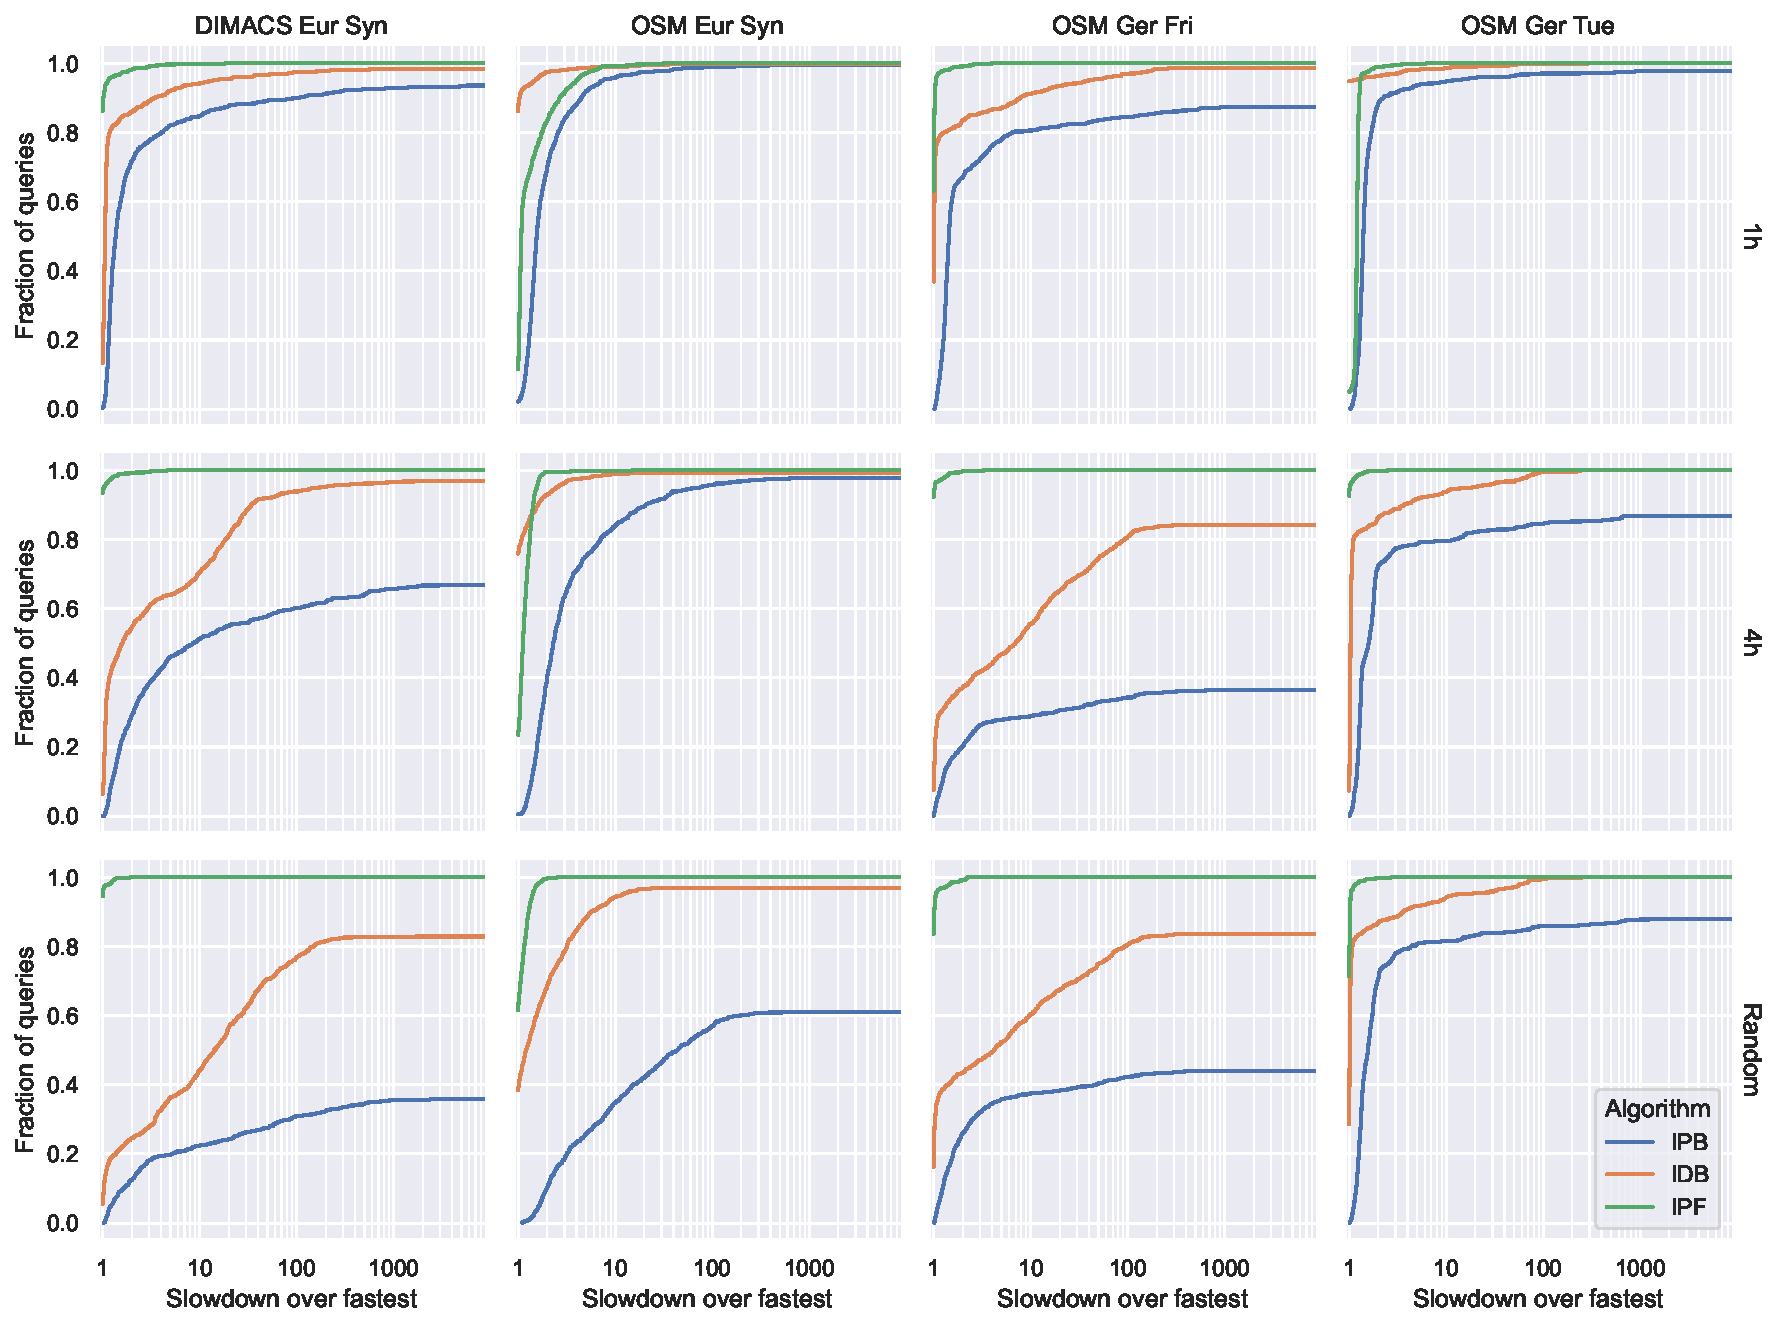
\includegraphics[width=.95\linewidth]{fig/detailed_perf_profile_time.pdf}
\caption{
Relative performance profile for the running time of our algorithms on all queries from Table~\ref{tab:data} split by graph and query set.
}\label{fig:perf_profile_time}
\end{figure}

\begin{figure}
\centering
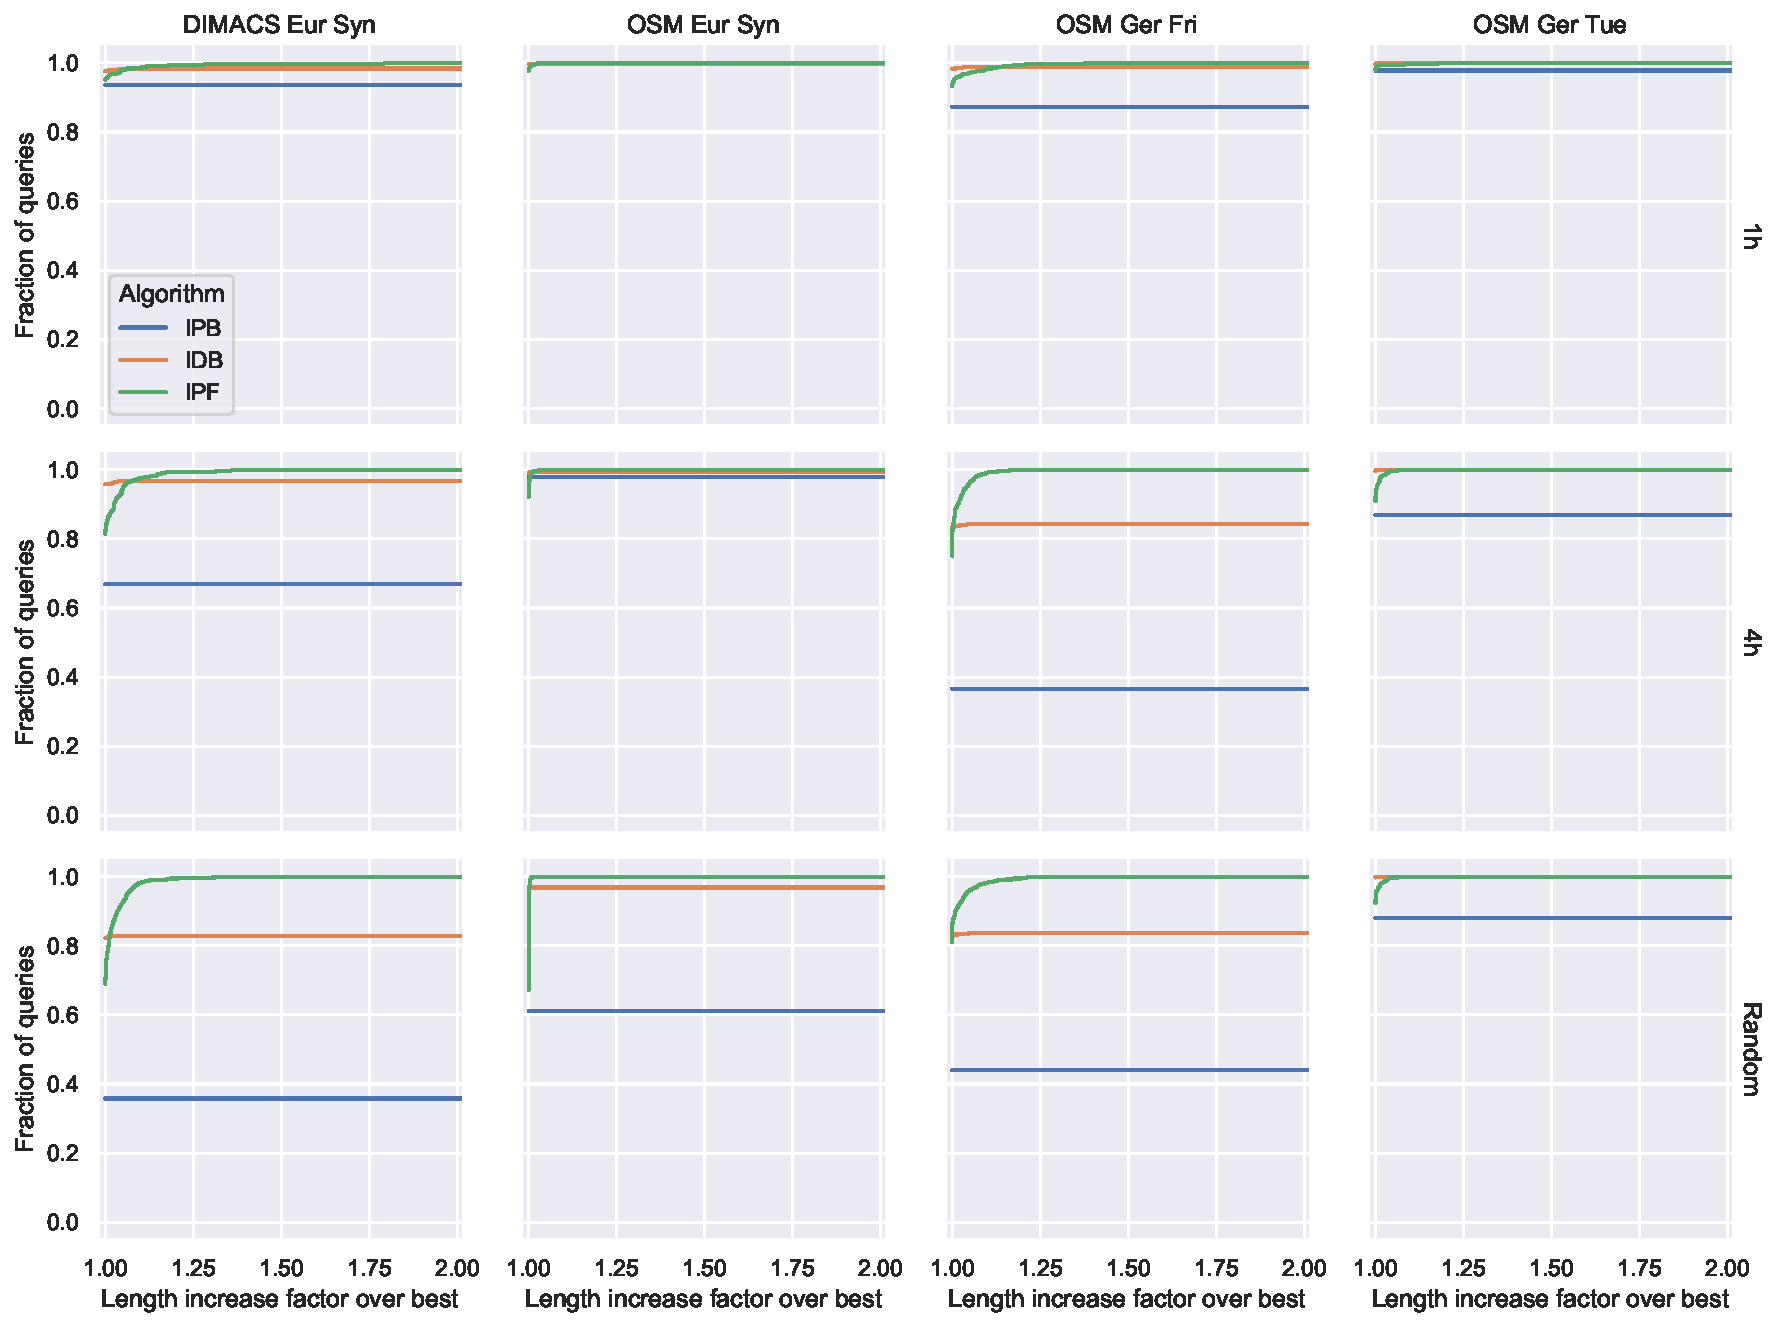
\includegraphics[width=.95\linewidth]{fig/detailed_perf_profile_quality.pdf}
\caption{
Relative performance profile for solution quality of our algorithms on all queries from Table~\ref{tab:data} split by graph and query set.
}\label{fig:perf_profile_quality}
\end{figure}

% \section{Styles of lists, enumerations, and descriptions}\label{sec:itemStyles}

% List of different predefined enumeration styles:

% \begin{itemize}
% \item \verb|\begin{itemize}...\end{itemize}|
% \item \dots
% \item \dots
% %\item \dots
% \end{itemize}

% \begin{enumerate}
% \item \verb|\begin{enumerate}...\end{enumerate}|
% \item \dots
% \item \dots
% %\item \dots
% \end{enumerate}

% \begin{alphaenumerate}
% \item \verb|\begin{alphaenumerate}...\end{alphaenumerate}|
% \item \dots
% \item \dots
% %\item \dots
% \end{alphaenumerate}

% \begin{romanenumerate}
% \item \verb|\begin{romanenumerate}...\end{romanenumerate}|
% \item \dots
% \item \dots
% %\item \dots
% \end{romanenumerate}

% \begin{bracketenumerate}
% \item \verb|\begin{bracketenumerate}...\end{bracketenumerate}|
% \item \dots
% \item \dots
% %\item \dots
% \end{bracketenumerate}

% \begin{description}
% \item[Description 1] \verb|\begin{description} \item[Description 1]  ...\end{description}|
% \item[Description 2] Fusce eu leo nisi. Cras eget orci neque, eleifend dapibus felis. Duis et leo dui. Nam vulputate, velit et laoreet porttitor, quam arcu facilisis dui, sed malesuada risus massa sit amet neque.
% \item[Description 3]  \dots
% %\item \dots
% \end{description}

% \cref{testenv-proposition} and \autoref{testenv-proposition} ...

% \section{Theorem-like environments}\label{sec:theorem-environments}

% List of different predefined enumeration styles:

% \begin{theorem}\label{testenv-theorem}
% Fusce eu leo nisi. Cras eget orci neque, eleifend dapibus felis. Duis et leo dui. Nam vulputate, velit et laoreet porttitor, quam arcu facilisis dui, sed malesuada risus massa sit amet neque.
% \end{theorem}

% \begin{lemma}\label{testenv-lemma}
% Fusce eu leo nisi. Cras eget orci neque, eleifend dapibus felis. Duis et leo dui. Nam vulputate, velit et laoreet porttitor, quam arcu facilisis dui, sed malesuada risus massa sit amet neque.
% \end{lemma}

% \begin{corollary}\label{testenv-corollary}
% Fusce eu leo nisi. Cras eget orci neque, eleifend dapibus felis. Duis et leo dui. Nam vulputate, velit et laoreet porttitor, quam arcu facilisis dui, sed malesuada risus massa sit amet neque.
% \end{corollary}

% \begin{proposition}\label{testenv-proposition}
% Fusce eu leo nisi. Cras eget orci neque, eleifend dapibus felis. Duis et leo dui. Nam vulputate, velit et laoreet porttitor, quam arcu facilisis dui, sed malesuada risus massa sit amet neque.
% \end{proposition}

% \begin{conjecture}\label{testenv-conjecture}
% Fusce eu leo nisi. Cras eget orci neque, eleifend dapibus felis. Duis et leo dui. Nam vulputate, velit et laoreet porttitor, quam arcu facilisis dui, sed malesuada risus massa sit amet neque.
% \end{conjecture}

% \begin{observation}\label{testenv-observation}
% Fusce eu leo nisi. Cras eget orci neque, eleifend dapibus felis. Duis et leo dui. Nam vulputate, velit et laoreet porttitor, quam arcu facilisis dui, sed malesuada risus massa sit amet neque.
% \end{observation}

% \begin{exercise}\label{testenv-exercise}
% Fusce eu leo nisi. Cras eget orci neque, eleifend dapibus felis. Duis et leo dui. Nam vulputate, velit et laoreet porttitor, quam arcu facilisis dui, sed malesuada risus massa sit amet neque.
% \end{exercise}

% \begin{definition}\label{testenv-definition}
% Fusce eu leo nisi. Cras eget orci neque, eleifend dapibus felis. Duis et leo dui. Nam vulputate, velit et laoreet porttitor, quam arcu facilisis dui, sed malesuada risus massa sit amet neque.
% \end{definition}

% \begin{example}\label{testenv-example}
% Fusce eu leo nisi. Cras eget orci neque, eleifend dapibus felis. Duis et leo dui. Nam vulputate, velit et laoreet porttitor, quam arcu facilisis dui, sed malesuada risus massa sit amet neque.
% \end{example}

% \begin{note}\label{testenv-note}
% Fusce eu leo nisi. Cras eget orci neque, eleifend dapibus felis. Duis et leo dui. Nam vulputate, velit et laoreet porttitor, quam arcu facilisis dui, sed malesuada risus massa sit amet neque.
% \end{note}

% \begin{note*}
% Fusce eu leo nisi. Cras eget orci neque, eleifend dapibus felis. Duis et leo dui. Nam vulputate, velit et laoreet porttitor, quam arcu facilisis dui, sed malesuada risus massa sit amet neque.
% \end{note*}

% \begin{remark}\label{testenv-remark}
% Fusce eu leo nisi. Cras eget orci neque, eleifend dapibus felis. Duis et leo dui. Nam vulputate, velit et laoreet porttitor, quam arcu facilisis dui, sed malesuada risus massa sit amet neque.
% \end{remark}

% \begin{remark*}
% Fusce eu leo nisi. Cras eget orci neque, eleifend dapibus felis. Duis et leo dui. Nam vulputate, velit et laoreet porttitor, quam arcu facilisis dui, sed malesuada risus massa sit amet neque.
% \end{remark*}

% \begin{claim}\label{testenv-claim}
% Fusce eu leo nisi. Cras eget orci neque, eleifend dapibus felis. Duis et leo dui. Nam vulputate, velit et laoreet porttitor, quam arcu facilisis dui, sed malesuada risus massa sit amet neque.
% \end{claim}

% \begin{claim*}\label{testenv-claim2}
% Fusce eu leo nisi. Cras eget orci neque, eleifend dapibus felis. Duis et leo dui. Nam vulputate, velit et laoreet porttitor, quam arcu facilisis dui, sed malesuada risus massa sit amet neque.
% \end{claim*}

% \begin{proof}
% Fusce eu leo nisi. Cras eget orci neque, eleifend dapibus felis. Duis et leo dui. Nam vulputate, velit et laoreet porttitor, quam arcu facilisis dui, sed malesuada risus massa sit amet neque.
% \end{proof}

% \begin{claimproof}
% Fusce eu leo nisi. Cras eget orci neque, eleifend dapibus felis. Duis et leo dui. Nam vulputate, velit et laoreet porttitor, quam arcu facilisis dui, sed malesuada risus massa sit amet neque.
% \end{claimproof}

\end{document}
